\documentclass[output=paper]{langsci/langscibook} 
\author{%
	Robert D.\ Borsley\affiliation{University of Essex and Bangor University}%
	\lastand Stefan Müller\affiliation{Humboldt-Universität zu Berlin}%
}
\title{HPSG and Minimalism}
\abstract{This chapter compares work done in Head-Driven Phrase Structure Grammar with work done under
  the heading \emph{Minimalist Program}. We discuss differences in the respective approaches and the 
  outlook of theories. We have a look at the procedural/""constraint"=based views on grammar and
  discuss the differences in complexity of the structures that are assumed. We also address psycholinguistic issues like processing and language acquisition.}

% \chapterDOI{} %will be filled in at production

\maketitle

\begin{document}

\label{chap-minimalism}

\section{Introduction}
\label{sec:min-intro}


The Minimalist\is{Minimalism|(} framework, which was first outlined by Chomsky in the early 1990s
\citep{Chomsky93b-u,Chomsky95a-u}, still seems to be the dominant approach in theoretical syntax. It is
important, therefore, to consider how HPSG compares with this framework. In a sense both frameworks
are descendants of the transformation"=generative approach to syntax, which Chomsky introduced in the
1950s. HPSG is a result of the questioning of transformational analyses\footnote{%
By \emph{transformational analyses} we mean analyses which derive structures from structures, especially
by movement, whether the movement is the product of transformational rules, a general license to
move, or the internal merge mechanism. 

We make no attempt to provide an introduction to HPSG in this chapter. For an introduction to the
various aspects of the framework, see the other chapters of this handbook. For example,
non-transformational analyses of the passive are dealt with in \crossrefchaptert{lexicon},
constituent order in \crossrefchaptert{order}, unbounded dependencies in \crossrefchaptert{udc}. The
question of whether scrmabling, passive, and nonlocal dependencies should be handled by the same
mechanism (\eg transformations) or whether these phenomena are distinct and should be analyzed by
making use of different mechanisms is discussed in \citew[Chapter~20]{MuellerGT-Eng3}.%
} that emerged in the late
1970s. This led to \isi{Lexical Functional Grammar} \citep{BK82a} and \isi{Generalized Phrase Structure Grammar} \citep{GKPS85a}, and then in
the mid 1980s to HPSG (\citealt{ps}, see \crossrefchaptert{evolution} for more on the origins of HPSG). Minimalism in contrast
remains committed to transformational, i.e. movement, analyses. It is simpler in some respects than
the earlier Government and Binding framework \citep{Chomsky81a}, but as we will see below, it involves a variety of
complexities. 

The relation between the two frameworks is clouded by the discourse that surrounds Minimalism. At one
time ``virtual conceptual necessity'' was said to be its guiding principle. A little later, it was
said to be concerned with the ``perfection of language'', with ``how closely human language approaches
an optimal solution to design conditions that the system must meet to be usable at all''
\citep[58]{Chomsky2002a-u}. Much of this discourse seems designed to suggest that Minimalism is quite
different from other approaches and should not be assessed in the same way. In the words of \citet[\page 19]{Postal2003a}, it
looks like ``an attempt to provide certain views with a sort of privileged status, with the goal of
placing them at least rhetorically beyond the demands of serious argument or evidence''. However, the
two frameworks have enough in common to allow meaningful comparisons.  


Both frameworks seek to provide an account of what is and is not possible both in specific languages and in language in general. Moreover, both are concerned not just with local relations such as that between a head and its complement or complements but also with non-local relations such as those in the following:
\eal
\ex\label{ex:min-student-knows}
The student knows the answer.
\ex\label{ex:min-raining}
It seems to be raining.
\ex\label{ex:min-which-student}
Which student do you think knows the answer? 
\zl
In (\ref{ex:min-student-knows}), \emph{the student} is subject of \emph{knows} and is
responsible for the fact that \emph{knows} is a third person singular form, but \emph{the student}
and \emph{knows} are not sisters if \emph{knows} and \emph{the answer} form a VP. In (\ref{ex:min-raining}) the subject
is \emph{it} because the complement of \emph{be} is \emph{raining} and \emph{raining} requires an
expletive subject, but \emph{it} and \emph{raining} are
obviously not sisters. Finally, in (\ref{ex:min-which-student}), \emph{which student} is
understood as the subject of \emph{knows} and is responsible for the fact that it is third person
singular, but again the two elements are structurally quite far apart. Both frameworks provide
analyses for these and other central syntactic phenomena, and it is quite reasonable to compare them
and ask which is the more satisfactory.\footnote{%
As noted below, comparison is complicated somewhat by the fact that Minimalists typically provide
only sketches of analyses in which various details are left quite vague.

We make no attempt to provide an introduction to HPSG in this chapter. For an introduction to the various aspects of the framework, see the other chapters of this handbook.}%

Although HPSG and Minimalism have enough in common to permit comparisons, there are obviously many differences. Some are more important than others, and some relate to the basic approach and outlook, while others concern the nature of grammatical systems and syntactic structures. In this chapter we will explore the full range of differences.

The chapter is organized as follows: in Section~\ref{sec:min-difference}, we look at differences of
approach between the two frameworks. Then in Section~\ref{sec:min-views-grammar}, we consider the
quite different views of grammar that the two frameworks espouse, and in
Section~\ref{sec:min-views-structure}, we look at the very different syntactic structures which
result. Finally, in Section~\ref{sec-psycho}, we consider how the two frameworks relate to
psycholinguistic issues, especially processing and language acquisition.

\section{Differences of approach and outlook}
\label{sec:min-difference}

%\inlinetodostefan{add brief intro}
This section deals with some higher level differences between the two frameworks. We start with the degree of
formalization and the range of data that is covered
(Section~\ref{sec-form-exhaust}). Section~\ref{sec-empirical-quality} discusses the quality of
empirical work. Finally, Section~\ref{sec-empty-els-innate-knowledge} deals with arguments for invisible entities and innate knowledge.

%% \subsection{Sociological differences}
%% \label{sec-sociological-differences}
%% A difference between Mainstream Generative Grammar\footnote{%
%%   We follow \citet[\page 3]{CJ2005a} in using the term \emph{Mainstream Generative Grammar} (MGG) to
%%   refer to work in Minimalism and the earlier Government \& Binding framework.%
%% } and HPSG that should not be underestimated is the fact that MGG has one
%% very important key figure, the by far most-cited linguist (and scientist in general) Noam
%% Chomsky. HPSG is different. This is how Carl Pollard put it:
%% \begin{quote}
%% There is no Chomsky-like figure who is always assumed to be basically on the right track no matter
%% what s/he proposes. HPSG research is normal science: the testing of hypothesies that appear
%% plausible given accepted assumptions. The goal is not to fill in the details of a vague theory which
%% is assumed to be basically right, but to successively replace empirical hypothesis with ones that
%% make better predictions. \citep[Section~1.2.1]{Pollard1997a}
%% \end{quote}
%% While Ivan Sag is perceived as the leading figure by outsiders, the fact that Ivan Sag's recent
%% switch to Sign-Based Construction Grammar\indexsbcg \citep{Sag2012a} is not unanimously adopted by
%% the HPSG community (see \crossrefchaptert{cxg} and \citew[Section~10.6.2]{MuellerGT-Eng2} for
%% discussion), that empty elements\is{empty element} are assumed by various researchers
%% \citep{Bender2000a,Mueller2004e,Borsley2009a-u} even though Ivan Sag argued
%% against them from 1994 \citep{SF94a} and that defaults\is{default} are not used by all researchers even though they play a
%% prominent role in Ivan Sag's work (\eg in \citealt{GSag2000a-u}) shows that Pollard's
%% claim is correct. Of course Ivan Sag is the most influential HPSG grammarian but this influence is
%% based on properly argued empirically interesting research.
%% \subsection{Stability vs. ``revolutions''}
%%
%% One other important difference is the stability of the framework. The formal machinery was in place
%% in the mid 80ies and the way it can be used was systematically explored in the decades to
%% come. This differs from MGG where several rather radical interruptions happened, the most noticable
%% being the one from Government \& Binding to Minimalism in the 90ies \citep*{LLJ2000a}.\todostefan{more?}
%%
%% Has Minimalism changed till the 90ies?


\subsection{Formalization and exhaustivity}
\label{sec-form-exhaust}

As many of the chapters in this volume emphasize, HPSG is a framework which places considerable
emphasis on detailed formal analyses of the kind that one might expect within Generative
Grammar.\footnote{%
We follow \citet[\page 2]{GSag2000a-u} in counting HPSG among Generative Grammar in the sense it was
defined by \citet[\page 4]{Chomsky65a}, namely as a framework that provides an explicit
characterization of the theories developed within it.
%CxG \citep*[\page 501]{FKoC88a}
When we refer to work in Government \& Binding or Minimalism, we follow \citet[\page 3]{CJ2005a} in using
the term \emph{Mainstream Generative Grammar}. It should be kept in mind that there is another
meaning associated with the term \emph{generative}. A generative grammar in the latter sense
generates a set (\citealp[\page 13]{Chomsky57a}. HPSG is not generative in this sense but rather model-theoretic. See \citet{PS2001a}
for differences between generative-enumerative and model theoretic approaches. See also
\crossrefchaptert{formal-background} and \crossrefchaptert{processing}.
}
Thus, it is not uncommon to find lengthy appendices setting out formal analyses. See, for
example, \citegen{Sag97a} paper on \ili{English} relative clauses\is{relative clause},
\citegen{VanEynde2015a-u} book on predicative constructions and especially \citet{GSag2000a-u},
which has a 50 page appendix. One consequence of this is that HPSG has had 
considerable influence in \isi{computational linguistics}. Sometimes theoretical work comes paired
with computer implementations, which show that the analyses are consistent and complete (\eg all
publications coming out of the \isi{CoreGram} project \citep{MuellerCoreGram} and the HPSG textbook
for German that comes with implementations corresponding to the individual chapters of the book
\citep{MuellerGrammix}). It has been noticed both by theorietical linguists \citep[\page 163]{Bierwisch63a} and
by theoretically oriented computational linguists \citep[\page 20]{Abney96a} that the interaction of phenomena
is so complex that most normal human beings cannot deal with this complexity and formalization and
implementation actually helps enormously to understand language in its full depth. For more on the
relation of HPSG and computational linguistics see \crossrefchapterw{cl}.



In Minimalism things are very different. Detailed formal analyses are virtually non-existent. There
appear to be no appendices like those in \citet{Sag97a} and \citet{GSag2000a-u}. In fact the
importance of \isi{formalization} has long been downplayed in Chomskyan work (\eg by Chomsky in an interview
with
%. Thus, in a 1980 conversation, Chomsky remarked that ``I do not see any point in formalizing for
%the sake of formalizing'' (see 
\citet[73]{HuybregtsRiemsdijk.1982} and in discussions between \citet{Pullum89b} and \citet[\page 146]{Chomsky90a}),
and this view seems fairly standard within Minimalism (see also the discussion in \citew[Section~3.6.2]{MuellerGT-Eng1}). \citet[\page 28]{CL95a-u}
attempt to justify the absence of detailed analyses when they suggest that providing a rule 
system from which some set of phenomena can be derived is not ``a real result'' since ``it is often
possible to devise one that will more or less work''. Instead, they say, ``the task is now to show how
the phenomena [\ldots] can be deduced from the invariant principles of \ug with parameters set in one
of the permissible ways''. 
%In other words, providing detailed analyses is a job for unambitious
%drudges, while real linguists pursue a more ambitious agenda. 
\citet[5]{Postal2004a-u} comments that
what we see here is the ``notion that descriptive success is not really
that hard and so not of much importance''. He points out that if this were true, one would expect
successful descriptions to be abundant within transformational frameworks. He argues that actual
transformational descriptions are quite poor, and justifies this assessment with detailed
discussions of Chomskyan work on strong crossover phenomena and passives in Chapters 7 and 8 of his
book. 

There has also been a strong tendency within Minimalism to focus on just a subset of the facts in
whatever domain is being investigated. As \citet[535]{CJ2005a} note, ``much of the fine detail of
traditional constructions has ceased to garner attention''. This tendency has sometimes been
buttressed by a distinction between \isi{core grammar}, which is supposedly a fairly straightforward
reflection of the language faculty, and a \isi{periphery} of marked constructions, which are of no great
importance and which can reasonably be ignored. However, as \citet{Culicover99a-u} and others have
argued, there is no evidence for a clear cut distinction between core and periphery. It follows that
a satisfactory approach to grammar needs to account both for such core phenomena as
\emph{wh}-interrogatives, relative clauses, and passives but also with more peripheral phenomena
such as the following: 
\eal
\ex It's amazing the people you see here.\label{ex:min-amazing-people}
\ex The more I read, the more I understand.\label{ex:min-read-understand}
\ex Chris lied his way into the meeting.\label{ex:min-chris-meeting}
\zl 
These exemplify the nominal extraposition construction (\citealt{ML96a}), the \isi{comparative
  correlative construction} \citep{CJ99a-u,Borsley2011a-u}, and
the \emph{X's Way} construction \citep{Salkoff88a-u,Sag2012a}. As has been emphasized in other
chapters, the HPSG system of types and constraints is able to accommodate broad linguistic
generalizations and highly idiosyncratic facts and everything in between. 

The general absence in Minimalism of detailed formal analyses is quite important. It means that
Minimalists may not be fully aware of the complexity of the structures they are committed to and
this allows them to sidestep the question whether it is really justified. It also allows them to avoid
the question of whether the very simple conception of grammar that they favour is really
satisfactory. Finally, it may be that they are unaware of how many phenomena remain unaccounted
for. These are all important matters.  

The general absence of detailed formal analyses has also led to Minimalism having little impact on
computational linguistics. There has been some work that has sought to implement Minimalist ideas
\citep{Stabler2001a,FG2012a,Fong2014a}, but Minimalism has not had anything like the productive
relation with computational work that HPSG has enjoyed (see \crossrefchaptert{cl} on computational
work in HPSG). Existing Minimalist implementations are rather toy
grammars analyzing very simple sentences, some are not faithful to the theories they are claimed to
be implementing,\footnote{%
  Fong's grammars are simple Definite Clause Grammars, that is, context-free phrase structure grammars, and hence nowhere near an implementation of
  Minimalism, contrary to claims by \citet*[\page 1221]{BPYC2011a}.
  Lin's parsers PrinciPar and MiniPar \citeyearpar{Lin93a,Lin2003a-u} are based on GB and Miniamlism
  but according to \citet[\page 116]{Lin93a} and \citet[\page 2487]{TSSC2019a}, they
  are not transformational but use a \slasch passing mechanism like the one developed in GPSG
  \citep{Gazdar81a} and standardly used in HPSG (see \crossrefchapteralp{udc}).
} and some do not even parse natural language but require pre-segmented, pre-formatted
input. For example, Stabler's test sentences have the form as in (\mex{1}).
\eal
\ex the king will -s eat
\ex the king have -s eat -en
\ex the king be -s eat -ing
\ex the king -s will -s have been eat -ing the pie
\zl
See \citet[Section~4.7.2]{MuellerGT-Eng3} for discussion. Torr implemented a large-scale grammar
\citep[\page 2487]{TSSC2019a}, but he also uses a \slasch passing mechanism and ``around 45''
versions of Move and Merge (p.\,2488) in comparison to the two versions usually assumed in
Minimalism (Move and Merge or Internal and External Merge). Torr's work cannot be discussed here in 
detail due to space limitations but a discussion will be part of the next edition of Müller's
grammatical theory textbook.


Summing up: The fact that certain variants of Minimalism share properties with Categorial Grammar
has been noticed early on \citep{BE95a}. Directional Minimalist Grammars were compared to CG and HPSG
by \citet{MuellerUnifying}. MGs were extended to include GPSG-style \slasch passing mechanisms by
\citet{Kobele2008a} and continue to use them in the versions of \citet{TS2016a}. We believe that
this work is fruitful and well-formalized but formalization is insufficient for most of the work in
Minimalism and idea from other frameworks are ignored more often than not.

\subsection{Empirical quality}
\label{sec-empirical-quality}

There are, then, issues about the quantity of data that is considered in Minimalist work. There are
also issues about its quality \citep{Schuetze2016a}. Research in HPSG is typically quite careful about data and often
makes use of corpus and experimental data (see for example
\citealt*{AA2017a-u,Mueller99a,Mueller2002b,BC2010a,MBC2012a,Chaves2013a-u,Miller2013a}; \citealt[Chapter~7]{VanEynde2015a-u};
\citealt{ACS2016a-u}; \citealt{SAHM2019a-u}
for examples of work with attested examples and for experimental\is{experiment} work).
This use of corpus data and attested examples is based on the insight that \isi{introspection} alone is not sufficient, given that an
enormous amount of time is spent to work out analyses and it would be unfortunate if these analyses
were built on a shaky empirical basis. See \citew{Mueller2007c} and \citew{MM2009a} for the
discussion of introspection vs.\ corpus data and \citew{HS2010a-u,GF2013a-u} for the discussion of introspection
vs.\ controlled experimental data.
Research in Minimalism is often rather less
careful.\footnote{
 We hasten to say that we do not claim this to be true for all Minimalist work. There are
 researchers working with corpora or at least with attested examples \citep{Wurmbrand2003a} and
 there is experimental work. Especially in Germany there were several large scale Collaborative
 Research Centers with a strong empirical focus which also fed back into theoretical work, including
 Minimalist work. The fact that we point out here is that there is work, including work
 by prominent Minimalists, that is rather sloppy as far as data is concerned.%
} In a review of a collection of Minimalist papers, \citet[\page 434]{Bender2002b-u} comments that: ``In
these papers, the data appears to be collected in an off-hand, unsystematic way, with unconfirmed
questionable judgments often used at crucial points in the argumentation''. She goes on to suggest
that the framework encourages ``lack of concern for the data, above and beyond what is unfortunately
already the norm in formal syntax, because the connection between analysis and data is allowed to be
remote.''. Similar things could be said about a variety of Minimalist work. Consider, for example,
\citet{AounLi.2003}, who argue for quite different analyses of \emph{that}-relatives and
\emph{wh}-relatives on the basis of the following (supposed) contrasts, which appear to represent
nothing more than their own judgements (p.\,110--112):
%\inlinetodostefan{dialectal variation}
\eal
\judgewidth{?*}
\ex[]{The headway that Mel made was impressive.}\label{ex:min-headway-that}
\ex[??]{The headway which Mel made was impressive.}\label{ex:min-headway-which}
\zl
\eal
\judgewidth{?*}
\ex[]{
We admired the picture of himself that John painted in art class.
}\label{ex:min-admire-that}
\ex[*]{
We admired the picture of himself which John painted in art class.
}\label{ex:min-admire-which} 
\zl
\eal
\judgewidth{?*}
\ex[]{The picture of himself that John painted in art class is impressive.}\label{ex:min-picture-that}
\ex[*?]{The picture of himself which John painted in art class is impressive.}\label{ex:min-picture-which} 
\zl
None of the native speakers we have consulted find significant contrasts here which could support
different analyses. The example in (\mex{1}a) with a \emph{which} relative clause referring to \emph{headway} can be found in
\citew{CHH82a-u}. \citew[\page 437]{Williams89a-u} and \citew[\page 221]{Falk2010a-u} have examples
with a reflexive coreferential with a noun in a relative clause introduced by \emph{which} as in
William's (\mex{1}b) and corpus examples like (\mex{1}c,d) can be found as well:
%\inlinetodostefan{BB: We need examples where a which relative has an antecedent containing a reflexive and the antecedent is inside the relative. Tom Wasow's examples look good to me.}
\ealnoraggedright
\ex The headway which we made was satisfactory.
\ex the picture of himself which John took

\ex The words had the effect of lending an additional clarity and firmness of outline to the picture
    of himself which Bill had already drawn in his mind--of a soulless creature sunk in hoggish
    slumber.\footnote{
      Wodehouse, P.G. 1917. \emph{Uneasy Money}, London: Methuen \& Co., p.\,186,
      \url{http://www.literaturepage.com/read.php?titleid=uneasymoney&abspage=186},
      2018-09-18.
}
\ex She refused to allow the 
picture of himself, which he had sent her, to be hung, 
and it was reported that she ordered all her portraits 
and busts of him to be put in the lumber attics.\footnote{
 Jerrold, Clare. 1913. \emph{The married life of Queen Victoria}, London: G.\ Bells \& Sons, Ltd.
 \url{https://archive.org/stream/marriedlifeofque00jerruoft/marriedlifeofque00jerruoft_djvu.txt}, 2018-09-19.
}
%% \ex The words had the effect of lending an additional clarity and firmness of outline to the picture
%% of himself which Bill had already drawn in his mind--of a soulless creature sunk in hoggish
%% slumber.\footnote{
%% Wodehouse, P.G. 1917. \emph{Uneasy money}. London: Methuen \& Co. \url{http://www.freeclassicebooks.com/P.G.\%20Wodehouse/Uneasy\%20Money.pdf}, 2018-09-19.
%% }

%% \ex Like Milton, Calvin believed that the scriptural presentation of God should be accepted as the
%%     picture of himself which God wished people to perceive \ldots\footnote{
%%   Neil D. Graves. 2001. \emph{Milton and the Theory of Accommodation}, Studies in Philology,
%%   Vol. 98, No. 2.
%% }
\zl
%Also in Yehuda N. Falk On the Syntactic Analysis of Relative Clauses
%
Given that it is relatively easy to come up with counterexamples it is surprising that authors do
not do a quick check before working out rather complex analyses.

Note that we are not just taking one bad example of Minimalist work. It is probably the case that
papers with dubious judgments can be found in any framework if only this is due to the repetitions
of unwarranted claims made by others. The point is that Aoun \& Li are influential (quoted by 455
other publications as of 2018-09-14). Others rely on these judgments or the analyses that were
motivated by them. New conclusions are derived from analyses since theories make predictions. If
this process continues for a while an elaborate theoretical edifice results that is not
empirically supported. Note furthermore that the criticism raised here is not the sqabble of two
authors working in an alternative framework. This criticism also comes from practitioners of
Mainstream Generative Grammar. For example, Wolfgang Sternefeld and Hubert Haider, both very
prominent figures in the German Generative Grammar school criticized the scientific standards in
Minimalism heavily \citep{%Ross2011a,
SR2012a,Haider2018a}. 
%% As \citet[\page 266--268]{SR2012a} point out it is not\todostefan{AA. Drop
%%   this paragraph}
%% just the case that Minimalist publications are based on empirically problematic foundations, it is
%% even worse: researchers like \citet[Section~1.1]{ES2006a-u} publish statements about research
%% methodology that can only be understood as an immunization strategy. The authors discuss the two
%% curves in Figure~\ref{fig-immunization-MP}:
%% one has a sine-like shape and hits three out of seven of the data points on a straight line and the
%% other one is parallel to the line with the data points and hence hits none of the data points. The
%% second approach gets none of the data right. Nevertheless the authors argue that one should prefer
%% this theory since it was closer to the truth and more illuminating: ``Clearly, Theory~1 is
%% `empirically preferable’ by a `winning score’ of 3--0. The point [\ldots] is that Theory~2, despite
%% getting none of the data correct, [\ldots] is `closer to the truth’ or `more illuminating’ than the
%% empirically preferable Theory~1. Hence, we believe, Theory~2 is a better working or guiding
%% hypothesis upon which to base future research.'' \citep[\page 2]{ES2006a-u}
%% \begin{figure}
%% \begin{subfigure}{0.48\textwidth}
%% \scalebox{.78}{%
%% \begin{tikzpicture}
%%     \begin{axis}[
%%         xmin=0,xmax=6,
%%         ymin=0,ymax=6,
%%         cycle list name=black white
%%     ]
%%     \addplot+ [sharp plot] coordinates {(0,0) (1,1) (2,2) (3,3) (4,4) (5,5) (6,6)};
%%     \addplot+ [smooth]     coordinates {(0,2.5) (1,1) (2,0.5) (3,3) (4,5.5) (5,5) (6,3.5)};
%%         \end{axis}
%% \end{tikzpicture}}
%% \caption{Theory 1}
%% \end{subfigure}
%% \hfill
%% \begin{subfigure}{0.48\textwidth}
%% \scalebox{.78}{%
%% \begin{tikzpicture}
%%     \begin{axis}[
%%         xmin=0,xmax=6,
%%         ymin=0,ymax=6,
%%         cycle list name=black white
%%     ]
%%     \addplot+ [sharp plot] coordinates {(0,0) (1,1) (2,2) (3,3) (4,4) (5,5) (6,6)};
%%     \addplot+ [sharp plot] coordinates {(0.2,0) (1,.8) (2,1.8) (3,2.8) (4,3.8) (5,4.8) (6,5.8)};
%%         \end{axis}
%% \end{tikzpicture}}
%% \caption{Theory 2}
%% \end{subfigure}
%% \caption{\label{fig-immunization-MP}Immunization in Minimalist work: According to \citet[Section~1.1]{ES2006a-u} Theory~2, which gets none of the data points, is
%%   preferable to Theory~1 with three data points since Theory~2 is ``more illuminating'' and ``closer to
%%   to the truth''}
%% \end{figure}

As we will show in Section~\ref{sec-labelling}, Minimalist discussions of the important topic of labelling have also
been marred by a failure to take account of relevant data. 

\subsection{Argumentation for invisible entities and the assumption of innate linguistic knowledge}
\label{sec-empty-els-innate-knowledge}

There are also differences in the kind of arguments that the two frameworks find acceptable. It is
common within Minimalism to assume that some phenomenon which cannot be readily observed in some
languages must be part of their grammatical system because it is clearly present in other
languages. Notable examples would be case \citep{Li2008a-u} or (object) agreement \citep[Chapter~4]{Meinunger2000a}, which are assumed to play a role
even though there are no visible manifestations within some languages (\eg \ili{Mandarin Chinese}
and \ili{German}, respectively). This stems from the longstanding Chomskyan 
assumption that language is the realization of a complex innate language faculty. From this
perspective, there is much in any grammatical system that is a reflection of the language faculty
and not in any simple way of the observable phenomena of the language in question. If some
phenomenon plays an important role in many languages it is viewed as a reflection of the language
faculty, and hence it must be a feature of all grammatical systems even those in which it is hard to
see any evidence for it. An example -- taken from a textbook on Minimalism \citep*[\page
  124]{HNG2005a} -- is an analysis of prepositional phrases in
English. Figure~\ref{fig-understnading-Minimalism-PP} shows the analysis.\footnote{%
  This analysis is actually a much simpler variant of the PP analysis which appeared in an earlier
  textbook by \citet[\page 452]{Radford97a-u}. For discussion of this analysis see \citet[\page
    549--550]{Sternefeld2006a-u} and \citet[Section~4.6.1.2]{MuellerGT-Eng1}. We are aware of the
  fact that Minimalism developed further since 1997 and 2005 and that some Agr projections are replaced
  by other mechanism, but first this is not true for all analyses (see for example
  \citew{Carnie2013a-u}) and second the way it is argued for analyses did not change.%
}
\begin{figure}
\hfill
\begin{forest}
sm edges
[AgrP
  [DP [me$_j$]]
  [Agr$'$
    [Agr [with$_j$]]
    [PP
      [P$'$
        [P [\trace$_i$]]
        [DP [\trace$_j$]]]]]]
\end{forest}
\hfill
\begin{forest}
[PP
  [P [with]]
  [NP [me]]]
\end{forest}
\hfill\mbox{}
\caption{\label{fig-understnading-Minimalism-PP}Minimalist analysis of a PP according to
  \citep*[\page 124]{HNG2005a} and the analysis assumed in HPSG and all other phrase structure-based frameworks}
\end{figure}
Due to theory internal assumptions the case requirement of the preposition cannot be checked in the
P-DP combination. According to the version of the theory adopted by the authors, case has to be
checked in specifier positions. Therefore it was assumed that the preposition moves to an Agr head
and the DP moves to the specifier position of this Agr head. The problem is of course that DP and P
are in the wrong order now. However, the authors argue that this is the order that is manifested in
\ili{Hungarian} and that Hungarian is a language which has postpositions and these are agreeing with
their nominal dependent. The authors assume that Hungarian postpositions are prepositions
underlyingly and that the DP following the preposition moves to the left because of a movement
process that is triggered by agreement. It is claimed that this movement exists both in Hungarian and in English but
that the movement is covert (that is, invisible) in the latter language.

This line of argument would be reasonable if a complex innate language
faculty were an established fact, but it isn't, and since \citet*{HCF2002a}, it seems to have been
rejected within Minimalism. It follows that ideas about an innate language faculty should not be
used to guide research on individual languages. Rather, as \citet[25]{MuellerCoreGram} puts it,
``grammars should be motivated on a language-specific basis''. Does this mean that other languages are
irrelevant when investigating a specific language? Clearly not. As \Citeauthor{MuellerCoreGram}
also puts it, ``In situations where more than one analysis would be compatible with a given dataset
for language X, the evidence from language Y with similar constructs is most welcome and can be used
as evidence in favor of one of the two analyses for language X.'' (\citeyear[43]{MuellerCoreGram}). In
practice, any linguist working on a new language will use apparently similar phenomena in other
languages as a starting point. It is important, however, to recognize that apparently similar
phenomena may turn out on careful investigation to be significantly different.\footnote{%
  Equally, of course, apparently rather different phenomena may turn out on careful investigation to
  be quite similar. For further discussion of HPSG and comparative syntax, see \citew{Borsley2018a}.%
} 

\section{Different views of grammar}
\label{sec:min-views-grammar}

We turn now to more substantive differences between HPSG and Minimalism, differences in their conceptions of grammar, especially syntax, and differences in their views of syntactic structure. As we will see, these differences are related. In this section we consider the former, and in the next we will look at the latter.

\subsection{Declarative and constraint-based vs.\ derivational and generative-enumerative approaches}

As is emphasized throughout this volume, HPSG assumes a declarative or constraint"=based view of
grammar. It also assumes that the grammar involves a complex systems of types and
constraints. Finally, it assumes that syntactic analyses are complemented by separate semantic and
morphological analyses. In each of these areas, Minimalism is different. It assumes a procedural
view of grammar. It assumes that grammar involves just a few general operations. Finally, it assumes
that semantics and morphology are simple reflections of syntax. We comment on each of these matters
in the following subsections. 

Whereas HPSG is a declarative or constraint-based approach, Minimalism seems to be firmly committed
to a procedural approach. \citet[219]{Chomsky95a-u} remarks that: ``We take L [a particular language]
to be a generative procedure that constructs pairs (π, λ) that are interpreted at the
articulatory-perceptual (A-P) and conceptual-intentional (C-I) interfaces, respectively, as
`instructions' to the performance systems.''. Various arguments have been presented within HPSG for
a declarative view, but no argument seems to be offered within Minimalism for a procedural
view. Obviously, speakers and hearers do construct representations and must have procedures that
enable them to do so, but this is a matter of performance, and there is no reason to think that the
knowledge that is used in \isi{performance} has a procedural character (see Section~\ref{sec-minimalism-processing} on processing). Rather, the fact that it is used in
both \isi{production} and \isi{comprehension} suggests that it should be neutral between the two and hence
declarative. See also \crossrefchaptert[Section~\ref{sec-processing-constraint-based}]{processing} on this point.

Another difference between constraint-based and generative-enumerative approaches is that the first
type of proposal provides a way to get graded acceptability into the picture \citep[Section~3.1]{PS2001a}. Since HPSG grammars
are basically feature-value pairs with equality (or other relations) between values, it is possible
to weigh constraints and it is possible to admit constraint violations and work with structures with
violated constraints (see for example \citealp{SK2005a} on cumulative constraint violation). So looking at the sentences in (\mex{1}) we see that more and more constraints
are violated:
\eal
\ex[]{
I am the chair of my department.
}
\ex[*]{
I are the chair of my department.
}
\ex[*]{
Me are the chair of my department.
}
\ex[*]{
Me are the chair of me’s department.
}
\ex[*]{
Me are chair the of me’s department.
}
\ex[*]{
Me are chair the me’s department of.
}
\zl

\noindent
In comparison to this a generative-enumerative grammar enumerates a set and a
sequence either is in the set or it is not.\footnote{%
For a discussion of Chomsky's
(\citeyear{Chomsky64a}; \citeyear[Chapter~5]{Chomsky75a}) proposals to deal with different degrees
of acceptability see \citew[\page 29]{PS2001a}.
}

%% Another interesting difference is the robustness of constraint-based models with respect to missing
%% information. If we hear utterances like (\mex{1}) we do not know the word \emph{dibbledidooed} but
%% we know many of its properties.
%% \ea
%% He dibbledidooed her the ball.
%% \z
%% The word must be a verb (because of its ending) and it must be ditransitive because of the
%% environment it occurs in. Since it is a ditransitive verb it is probably a verb the signals change
%% of possession. All this information follows from constraints imposed on the verb by the surrounding structure.

For further discussion of the issues, see Section~\ref{sec-minimalism-processing} of
this paper and e.\,g.\ \citet{PS2001a}, \citet{Postal2003a}, \citeauthor{SW2011a}
\citeyearpar{SW2011a,SW2015a}, and \crossrefchaptert{processing}.  

\subsection{Underspecification}

Another crucial difference between HPSG and Minimalism is that HPSG allows for the underspecification of
information. In the absence of constraints, all principle options are possible. This is different in
Minimalism. All structures that are derivable are predetermined by the numeration. Features have to
be specified and they determine movement and properties of the derived objects. The general
characterization of the frameworks is: 
\eal
\ex Minimalism: Only what is explicitly ruled in works. 
\ex HPSG: Everything that is not ruled out works.
\zl
Let us consider some examples. 
The availability of type hierarchies makes it possible to underspecify part-of-speech
information. For example, \citet{Sag97a} assumes that complementizer (\type{comp}) and verb
(\type{verb}) have a common supertype \type{verbal}. A head can then select for a complement with the category \type{verbal}. So rather
than specifying two lexical items with different valence information or one with a disjunctive
specification \type{verb} $\vee$ \type{comp}, one has just one lexical item selecting for
% Adger2003:294 empty comp
\type{verbal}. Similarly, schemata (grammar rules) can contain underspecified types. A daughter in a
dominance schema can have a value of a certain types that subsumes a number of other
types. Let's say three. Without this underspecification one would need three schemata: one for every
subtype of the more general type.

Quantifier scope can be underspecified as well (\citealp*{CFPS2005a}; \citealp{RS99c-u}; \crossrefchapteralp{semantics}): constraints regarding which quantifier outscopes
which other quantifier may be left unspecified. The absence of the respective constraints results
in a situation where several scopings are possible. In transformational models it is usually assumed
that quantifier elements move into certain positions covertly and scope relations are read off of
the resulting tree \citep{May85a-u,Frey93a,SE2002a}. This is unnecessary in HPSG. (see
p.\,\pageref{page-scrambling-scope} for wrong predictions of movement-based approaches to quantifier scope).
%% \footnote{%
%% Apart from the possibility of a more compact specification of scope relations, HPSG analyses are
%% actually superior on an empirical level. As \citet{Kiss2005a} and independently also
%% \citet{Fanselow2001a} (working in a Minimalist setting) have shown, movement"=based approaches
%% cannot account for cases in which two quantified noun phrases are moved simultaneously while
%% maintaining their relative order. Reconstruction predicts too many readings. \citet{SE2002a}
%% provided a solution to the problem but the analysis has an absurd complexity involving several
%% movements, some of them invisible. For more discussion of scrambling and scope and the approaches
%% mentioned here see \citew[\page 114--116]{MuellerGT-Eng3}.
%% }\todostefan{AA: drop footnote. It is too much. Stefan: Actually we discuss Sauerland later as well. We may
%%   reorganize things.}
%% Related to scope and scrambling is the fact that order does not have to be specified in dominance
%% schemata. While simple phrase structure rules determine the order of the elements on their
%% right"=hand side, dominance schemata in HPSG do not say anything about the order of their
%% daughters. Unless linearization constraints (LP rules) enforce a certain ordering, everything
%% goes. In comparison, traditional phrase structure grammars need six phrase structure rules to derive the
%% six orders of a verb"=final clause with a ditransitive verb in German and transformational
%% approaches needed a base-configuration and derived configurations (leading to the problems mentioned
%% above). HPSG needs only one schema. For more discussion and details on the actual analysis of German
%% word order with binary branching structures see \crossrefchaptert{order}.

%% Another example for underspecification The chapter on constituent order \crossrefchapterp[\page \pageref{schema-head-adjunct}]{order} discusses
%% the Head-Adjunct Schema. This schema says that head"=adjunct structures consist of a head and an
%% adjunct but it does not say anything about the order of the two daughters. If nothing else is said
%% (\eg in form of linearization constraints), this means that both orders of head and adjunct are
%% possible.\todostefan{Hey, but Merge is set-based and sets do not have any order.}



%% \inlinetodostefan{AA: this should be expanded since it is very important\newline
%% %
%% syntactic category can be underspecified, for example if one wants to
%%  define the sentence as headed by a verb or by a complementizer,  one can
%%  posit an underspecified category verbal which subsumes both, while in
%%  minimalism one has to choose between VP, IP, TP, CP etc.\newline
%% %
%%  word order can be underspecified (between complements of ditransitive
%%  verbs for instance, or between certain head and adjunct) without having
%%  to posit one basic order and derive the other (ref chapter constituent
%%  order), quantifier scope can be underspecified (ref chapter semantics) etc.}


\subsection{Types and constraints vs.\ general operations}
\label{sec-types-vs-operations}

The declarative-procedural contrast is an important one, but the contrast between the complex
systems of types and constraints that are assumed within HPSG and the few general operations that
form a Minimalist grammar is arguably more important.\footnote{%
  A procedural approach doesn't necessarily involve a very simple grammatical system. The Standard
  Theory of Transformational Grammar \citep{Chomsky65a} is procedural but has many different rules,
  both phrase structure rules and transformations.}
Much work in Minimalism has three main operations Merge, Agree, and Move or Internal Merge. Merge\is{Merge!External}
combines two expressions, either words or phrases, to form a larger expression with the same label
as one of the expressions \parencites[244]{Chomsky95a-u}[\page 140]{Chomsky2008a}. Its operation can be presented as shown in Figure~\ref{fig:min-merge}.
\begin{figure}
\centering
	\raisebox{1\baselineskip}{X, Y $\Rightarrow$}
	\hspace{1em}
	\begin{forest}
		[X [X] [Y]]
	\end{forest}
\hspace{1em}
\raisebox{1\baselineskip}{or}
\hspace{1em}
	\begin{forest}
		[Y [X] [Y]]
	\end{forest}
	\caption{\label{fig:min-merge}Merge}\is{Merge}
\end{figure}
In the case of English, the first alternative is represented by situations where a lexical head
combines with a complement while the second is represented by situations where a specifier combines
with a phrasal head. \citet[\page 146]{Chomsky2008a} calls items merged with the first variant of Merge \emph{first-merged}
and those merged with the second variant \emph{later-merged}.

Agree\is{Agree|(}, as one might suppose, offers an approach to various kinds of agreement phenomena. It involves
a \isi{probe}, which is a feature or features of some kind on head, and a goal, which the head
c-commands\is{c-command}.
%% \footnote{%
%%   It is not necessary to state the c-command restriction since it is assumed that linguistic objects are built
%%   bottom-up and when a head is combined with its dependent the head can ``see'' the dependent but
%%   not the context in which the resulting object is embedded. Information about dominating material
%%   will be available only later in the derivation. (Guido Mensching, p.\,c.\ 2018)%
%% }%\todostefan{\citew[\page 142]{Chomsky2008a} contrasts c-command with Agree} 
At least normally, the probe is a linguistic object with an uninterpretable feature or features with no value and
the goal has a matching interpretable feature or features with appropriate values \citep[\page
  3--5]{Chomsky2001a-u}.\footnote{%
 Chomsky also assumes that the goal also has an uninterpretable feature of some kind to render it 'active'. In the case of subject-verb agreement, this is a Case feature on the subject.
}
Agree values the uninterpretable feature or features and they are ultimately deleted, commonly after they have triggered some morphological effect. Agree can be represented as in Figure~\ref{fig:min-agree} (where the ``u'' prefix identifies a feature as uninterpretable, and we have just one uninterpretable feature on the probe and just one matching interpretable feature on the goal).
%% The goal also has an uninterpretable feature of some kind to render it ``active''. 
%% An example for such a feature is Case, which will be discussed in more detail below. 
%% Agree values the uninterpretable feature or features and they are ultimately deleted, commonly after they have
%% triggered some morphological effect. Agree can be represented as in Figure~\ref{fig:min-agree} (where the ``\textit{u}''
%% prefix identifies a feature as uninterpretable).
\begin{figure}
\centering
\begin{forest} 
%sm edges without translation, 
empty nodes
[{}
  [X \\ {[\textit{u}F1]}]
  [{}
    [Y \\ {~~[F1 v]~~~}, roof]]]
\end{forest}
\hspace{1em}
\raisebox{4\baselineskip}{$\Rightarrow$}
\hspace{1em}
\begin{forest}
%	sm edges without translation, 
empty nodes
	[{}
	[X \\ {[\textit{u}F1 v]}]
	[{}
	[Y \\ {\makebox[3em]{[F1 v]}}, roof]]]
\end{forest}
\caption{\label{fig:min-agree}Agree}\is{Agree}
\end{figure}
Unsurprisingly subject-verb agreement is one manifestation of Agree, where X is T(ense) and Y is a
nominal phase, for Minimalism a DP, inside the complement of T.\footnote{%
It is assumed within Minimalism that subjects originate inside the complement of T and that they are raised to the Specifier of T in English and many other languages.}
T presumably has two uninterpretable features, person and number, and the DP two matching interpretable features. Here, and elsewhere,
Agree is a non-local\is{locality} relation involving elements which are not sisters. This contrasts
with the situation in HPSG, in which subject-verb agreement is a consequence of a relation between
the subject and its VP sister and a relation between the VP and the V that heads it.\is{Agree|)}

Finally, Move\is{Move|(}, also called Internal Merge\is{Merge!Internal}, is an operation which makes a copy of a constituent of some
expression and merges it with the expression \parencites[Section~4.4]{Chomsky95a-u}[\page
  140]{Chomsky2008a}. The original element that is copied normally undergoes deletion. The process
can be presented as in Figure~\ref{fig:min-move}. 
\begin{figure}
\centering
\begin{forest} 
%		sm edges without translation, 
nice empty nodes
[{}
  [X]
  [{},tier=flat
    [{\makebox[3em]{Y}}, roof]]]
\end{forest}
\hspace{1em}
\raisebox{4\baselineskip}{$\Rightarrow$}
\hspace{1em}
\begin{forest}
%		sm edges without translation, 
nice empty nodes
[{}
  [Y]
  [{}
    [X]
    [{},tier=flat
      [{\makebox[3em]{\sout{Y}}}, roof]]]]
\end{forest}
\caption{\label{fig:min-move}Move}\is{Move}
\end{figure}

This covers both the A$'$-movement\is{movement!A$'$} process assumed for \isi{unbounded dependency} constructions
such as \emph{wh}-interrogatives\is{interrogative} and the A-movement\is{movement!A} process assumed for \isi{raising} sentences and
passives. A question arises about so"=called head"=movement, where a head moves to a higher head
position. This appears to mean that it must be possible for the copy to be merged with the head of
the expression that contains it. However, this is incompatible with the widely assumed \isi{extension
condition}, which requires Merge to produce a larger structure. One response is the idea espoused in
\citeauthor{Chomsky95b-u} (\citeyear[368]{Chomsky95b-u}; \citeyear[37]{Chomsky2001a-u}) that
head"=movement takes place not in the syntax but in the PF component, which maps syntactic
representations to phonetic representations. It seems that its status is currently rather unclear.\is{Move|)}

The three operations just outlined interact with lexical items to provide syntactic analyses. It follows that the properties of constructions must largely derive from the lexical items that they contain. Hence, the properties of lexical items are absolutely central to Minimalism. Oddly, the obvious implication – that the lexicon should be a major focus of research – seems to be ignored. As \citet[95, fn.\,9]{Newmeyer2005a} comments:
\begin{quote}
[\ldots] in no framework ever proposed by Chomsky has the lexicon been as important as it is in the
MP [Minimalist Program]. Yet in no framework proposed by Chomsky have the properties of the lexicon
been as poorly investigated. \citep[95, fn.\,9]{Newmeyer2005a}
\end{quote}
Sometimes it is difficult to derive the properties of constructions from the properties of visible
lexical elements. But there is a simple solution: postulate an invisible element. The result is a
large set of invisible\is{empty element} functional heads\is{head!functional}. As we will see in Section~\ref{sec-cartography}, these heads do the work in Minimalism that is done by phrase types and the constraints on them in HPSG.

Although Minimalism is a procedural approach and HPSG a declarative approach, there are some
similarities between Minimalism and early HPSG, the approach presented in \citet{ps,ps2}. In much
the same way as Minimalism has just a few general mechanisms, early HPSG had just a few general
phrase types. Research in HPSG in the 1990s led to the conclusion that this is too simple and that a
more complex system of phrase types is needed to accommodate the full complexity of natural language
syntax. Nothing like this happened within Minimalism, almost certainly because there was little
attempt within this approach to deal with the full complexity of natural language syntax. As noted
above, the approach has rarely been applied in detailed formal analyses. It looks too simple and it
appears problematic in various ways. It is also a major source of the complexity that is
characteristic of Minimalist syntactic structures, as we will see in Section~\ref{sec:min-views-structure}. 

%% \subsection{Feature-driven movement, cyclic movement, and infinite lexicons}

%% Minimalism standardly assumes that movement is feature-driven.\todostefan{add reference} For
%% example, the \emph{wh} element has a feature that triggers movement. So in (\mex{1}) the \emph{who}
%% may not stay in the object position of \emph{like} but has to move to the specifier position of
%% CP. This movement causes the deletion of the respective feature at the \emph{wh} element. Without
%% such a deletion, \emph{who} would have an unchecked feature and the derivation would ``crash at the
%% interfaces'' since the \emph{wh} feature cannot be interpreted.
%% \eal
%% \ex[*]{
%% Does Kim like who?
%% }
%% \ex[]{
%% Who does Kim like?
%% }
%% \zl
%% This whole machinery is a huge stipulation\todostefan{change} and it raises issues of language acquisition, but let us
%% assume this machinery for the sake of argumentation. \emph{wh} movement is an unbounded dependency,
%% so it can cross clause boundaries. Minimalism assumes (like GB and other variants of
%% Transformational Grammar before) that movement is cyclic. That is, the \emph{wh} item moves to the
%% specifier position of the CP \emph{that Kim likes}. From there it moves to the specifier position of
%% \emph{that Sandy believes that Kim likes} and from there to the top-most specifier position.
%% \ea
%% Who did Aicke claim that Sandy believes that Kim likes?
%% \z 
%% Now, the interesting thing is that the \emph{wh} feature of the \emph{wh} elements get checked when
%% it is moved. So if the \emph{wh} element has exactly one \emph{wh} feature, this is gone once the
%% item arrives in the first specifier position. For examples like the one in (\mex{0}) the \emph{wh}
%% item would need three \emph{wh} features. Chomsky claims that languages are infinite sets since it
%% would be arbitrary to impose restrictions on the number of possible embeddings. We do not
%% necessarily agree on the infinitude claims \parencites{PS2010a}{MuellerGT-Eng1}, but we agree that
%% there should not be any arbitrary limitations on embeddings in competence grammars. If one excepts
%% this it would not suffice that a \emph{wh} item is ambiguous in having one or two or three \emph{wh}
%% features. The \emph{wh} item would have to be infinitely many times ambiguous since the number of
%% \emph{wh} features should not be limited since limits would be arbitrary.

%% Bob: One view is that the heads that constitute all the intermediate positions are defective (lacking in some features) and therefore the feature that allows the moving constituent to move is not deleted. It is only deleted when it reaches its final position where there is a on-defective head. But there is probably a question about why a constituent woud move to a position which doesn't allow the deletion of a feature which needs to be deleted. 

%% Note that this results in an infinite lexicon. It is unclear how this is supposed to work without an
%% elaborate theory of the lexicon. HPSG has lexical rules so lexical items can be derived from more
%% basic lexical entries. No such thing exist in Minimalism. Of course one could assume special
%% mechanisms that reintroduce features after checking them and so enabling further movement but these
%% mechanisms would be further stipulations and again add to the problem of \isi{language acquisition}.

%% A further problem of feature-driven movement is what \citet{Fanselow2003b} called \emph{altruistic
%%   movement}\is{movement!altruistic}. Altruistic movement is movement of a constituent that happens
%% in order to make room for another constituent in a certain position. If a certain constituent is
%% moved out of the way, it does not have a focus feature or a topic feature that can be checked since
%% neither being topic nor being focus is the reason for moving the constituent. It is another
%% constituent that requires in a certain position and this is the reason for movement.

\subsection{Labelling}
\label{sec-labelling}

As we noted in the last section, Merge combines two expressions to form a larger expression with the
same label as one of the expressions. But which of the original expressions provides the label for
the larger expression? This issue has been discussed but not very satisfactorily.
%%
%% Another quite important example of ignoring relevant data is Chomsky's work on Labeling.\inlinetodostefan{As I say elsewhere I think any detailed discussion of labelling should be in section 3 though it seems reasonable to make the point here that the discussion of these issues has been marred by a failure to notice some fairly obvious examples. } Labeling is
%% concerned with the question of the category that results when two items are combined. As is
%% discussed in more detail below, Chomsky assumes that the combination of two items with the labels
%% X and Y has to be either X or Y. 
Chomsky defines which label is used in two different cases: the first case states that the label\is{labeling} is the
label of the head if the head is a lexical item and the second case states the label to be the
label of the category from which something is extracted \citep[\page 145]{Chomsky2008a}. 
As Chomsky notes, these rules are not unproblematic since the label is not uniquely determined in all
cases. An example is the combination of two lexical elements since in such cases both elements can
be the label of the resulting structure. Chomsky notices that this could result in deviant structures, but
claims that this concern is unproblematic and ignores it. This means that rather fundamental notions
in a grammar theory were ill-defined. A solution to this problem was provided in his
\citeyear{Chomsky2013a} paper (published five years later), but this paper is inconsistent
\citep[Section~4.6.2]{MuellerGT-Eng1}. But this inconsistency is not the point we want to focus on here. Rather
we want to show one more time that empirical standards are not met. Chomsky uses underdetermination
in his labeling rules to account for two possible structures in (\mex{1}), an approach going back to
\citew{Donati2006a-u}:
\ea
\label{ex-what-you-wrote}
what [ C [you wrote \emph{t}]]
\z
(\mex{0}) can be an interrogative clause as in \emph{I wonder what you wrote.} or a free relative
clause as in \emph{I will read what you wrote.}. According to the labeling rule that accounts for
sentences from which an item is extracted, the label will be CP since the label is taken from the
clause. However, since \emph{what} is a lexical item, \emph{what} can determine the label as
well. If this labeling rule is applied \emph{what you wrote} is assigned DP as a label and hence the
clause can function as a DP argument of \emph{read}. 

Chomsky's proposal is interesting but it does not extend to cases involving free relative clauses
with complex \emph{wh}"=phrases (so"=called \isi{pied-piping}) as they are attested in examples like
(\mex{1}): 
\eal
\ex I'll read [whichever book] you give me.
\ex He gave me [what money] he had.
\zl
The example in (\mex{0}a) is from one of the standard references on free relative clauses:
\citew[\page 333]{BG78}, which is also cited in other mainstream generative work as for example
\citep{GR81}. (\mex{0}b) is from \citew[\page 1068]{HPP2002a-u}, a descriptive grammar of English.

Apart from the fact that complex \emph{wh}"=phrases are possible there is even more challenging data in the area of
free relative clauses: the examples in (\mex{1}) and (\mex{2}) show that there are non-matching free
relative clauses:
\ea
\gll Sie kocht, worauf   sie Appetit  hat.\footnotemark\\
     she cooks  where.on she appetite has\\\hfill(German)
\footnotetext{
\citew[\page 154]{Bausewein90}.
}
\glt `She cooks what she feels like eating.'
\z
\eal
\ex
\gll Worauf man sich mit einer Pro-form beziehen kann, [\ldots]  ist eine Kon\-sti\-tu\-en\-te.\footnotemark\\
     where.upon one self with a Pro-form  refer   can  {}        is  a    constituent\\
%      {`What you can refer to with a Pro-form, [\ldots] is a constituent.'}
\footnotetext{%
        From the main text of: G{\"u}nther Grewendorf, {\em Aspekte der deutschen Syntax. Eine Rektions-Bindungs-Analyse}.
        Studien zur deutschen Grammatik, number 33. T\"ubingen: Gunter Narr Verlag. 1988, p.\,16, quoted from \citew[\page 61]{Mueller99b}.
      }
\glt `If you can refer to something with a Pro-form, [\ldots] it is a constituent.'
\ex
\gll {}[Aus wem] noch etwas herausgequetscht werden kann, ist sozial dazu ver\-pflich\-tet, es
abzuliefern; \ldots\label{bsp-droste}\footnotemark\\
  \spacebr{}out who yet something out.squeezed be can is socially there.to obliged it to.deliver\\
\footnotetext{%
        Wiglaf Droste, taz, 01.08.97, p.\,16, quoted from \citew[\page 61]{Mueller99b}.
      }\\
\glt `Those who have not yet been bled dry are socially compelled to hand over their last drop.'
\zl
In (\mex{-1}) a relative clause with a PP relative phrase functions as an accusative object. In
(\mex{0}) the relative clauses function as subjects. (\mex{0}b) is another example of a relative
clause with a complex \emph{wh} phrase. See \citet{Bausewein90} and \citet{Mueller99b} for further discussion of free relative
clauses and attested data.

According to \citet[Section~5]{Donati2006a-u}, pied piping does not
exist in free relatives  (see also \citew[\page 930--932]{Citko2008a} for a rejection of this
claim). Given how much attention the issue of Labeling has received and how central this is 
to Minimalist analyses this situation is quite surprising: an empirically false claim made in
2002/2003 at two high profile conferences is the basis for foundational work from 2002 until 2013 even though the facts are common knowledge
in the field. \citet{Ott2011a} develops an analysis in which the category of the relative phrase is
projected, but he does not have a solution for nonmatching free relative clauses, as he admits in a
footnote on page 187. The same is true for Citko's analysis \citeyearpar{Citko2008a}, in which the
extracted XP can provide the label. So, even though the data has been known for decades, it is ignored by
authors and reviewers and foundational work is built on shaky empirical ground. See
\citew[Section~4.6.2]{MuellerGT-Eng1} for a more detailed discussion of labeling.


%% This is nonsense since the uninterpretable feature is at the head. St. Mü. 26.08.2019
%%
%% No it is not. Adger really assumes that the noun(!) has the unvalued case feature. Maybe because
%% English usually has underspecified case.

\subsection{Feature deletion and ``crashing at the interfaces''}

In Section~\ref{sec-types-vs-operations}, we mentioned Case as an uninterpretable feature which
renders a DP active. Like other uninterpretable features this is deleted as a result of Agree
because it is not interpretable in LF. 
% David Adger Mail 04.09.2019
%% \inlinetodostefan{Stefan: check: The
%%   uninterpretable feature is at the head, but the noun has to be valued. What if the NP has a case
%%   value from morphology already? It has to be eaten up, hasn't it?} 
This means that Minimalism claims
that a case marked NP like \emph{der Mann} `the man' is not interpretable unless it is somehow
stripped of its case information.
%% \footnote{
%%   Note that the morphological information is needed for spelling-out the correct form.
%% }
So in Minimalism \emph{der Mann} needs something on top of the DP
that Agrees with and thereby consumes the case feature. While this seems cumbersome to most working outside Minimalism,
there are actually deeper problems connected to the deletion of case features. There are
situations in which you need case features more than once. An example of this is free relative
clauses as the one in (\mex{1}b):
\eal
\ex 
\gll der Mann\\
     the.\nom{} man\\
\ex
\gll Ich treffe, wen ich treffen will.\\
     I meet who.\acc{} I meet want.to\\
\glt `I meet whoever I like to meet.'
\zl
\emph{wen} is the accusative object in the relative clause. Since it is an object its case feature
will be checked by the selecting verb \emph{treffen} `meet'. \emph{wen} will then be a DP without
any case information. However, the case of the relative phrase in free relative clauses is not
arbitrary. It is important for the integration of the free relative clause in the matrix clause. The
case of \emph{wer} `who' in a complete relative clause has to be known since it is important for the
external distribution of the free relative clause, as the examples in (\mex{1}) show:
\eal
\ex[]{
\gll Wer mich treffen will, kann vorbeikommen.\\
     who.\nom{} me   meet    wants.to may over.come\\
\glt `He who wants to meet me may come over.'
}
\ex[*]{
\gll Ich treffe, wer mich treffen will.\\
     I meet      who.\nom{} me meet wants.to\\
\glt `I meet whoever wants to meet me.'
}
\zl
HPSG also consumes resources in a way: items in valence representations are not projected up the
tree once the requirement is saturated, but the difference is that objects with a certain structure
and with certain features are not modified. A case-marked NP is not deprived of this case
information. We think that this is the right way to deal with morphological
markings and with feature specifications in general.

\subsection{Some implications}

We will look in detail at the implications for syntactic structure of this machinery in the next
section. However, we will note some implications in the following paragraphs as a kind of preview of the next section.

First, the fact that Merge combines two expressions entails that syntactic structures are confined
to binary branching\is{branching!binary} and excludes various analyses that have been assumed within
HPSG and other frameworks. Second, the assumption that expressions produced by Merge have the same
label as one of the expressions that they consist of \citep[\page 145]{Chomsky2008a} is essentially the assumption that all complex
expressions are headed\is{head}. For HPSG, as for many other approaches, there are headed expressions and
non-headed expressions, \eg coordination and the \isi{NPN construction} discussed in
Sections~\ref{sec-coordination-minimalism} and~\ref{sec-npn-minimalism}, respectively.

As emphasized above, a further important feature of Minimalism is the view that semantics and
morphology are simple reflections of syntax. The basic architiecture assumed in Minimalism is shown
in Figure~\ref{fig-architecture-phases}. Both phonology and semantics are read off the structures
produced by syntax.
\begin{figure}
\hfill
\scalebox{.92}{%
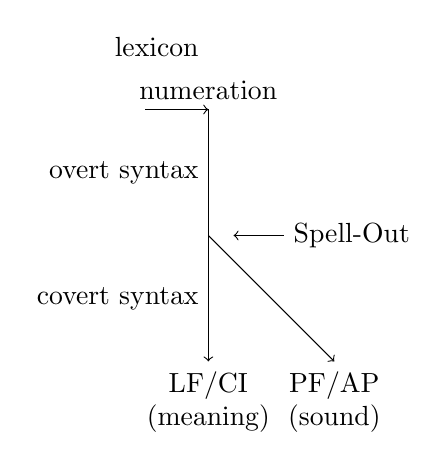
\begin{tikzpicture}[scale=.8,baseline=(current bounding box.center)]
%\draw (-2.9,-5.8) to[grid with coordinates] (2.7,-0.6);
\draw[->] node[anchor=east] {lexicon} (-1,-1) -- (0,-1); 
\draw[->] (0,-1) node[anchor=south] {numeration} --(0,-5) node[anchor=north, align=center] {LF/CI\\(meaning)};
\draw[->] (0,-3)--(2,-5) node[anchor=north,align=center] {PF/AP\\(sound)};
\draw[<-] (.4,-3)--(1.2,-3) node[anchor=west] {Spell-Out};
%\draw (0,-0.5) node {lexicon};
%\draw (-2.9,-2) node[anchor=west] {overt syntax};
%\draw (-2.9,-4) node[anchor=west] {covert syntax};
\draw (-.0,-2) node[anchor=east] {overt syntax};
\draw (-.0,-4) node[anchor=east] {covert syntax};
%\draw (0,-6.5) node[align=center] {LF/CI\\(meaning)};
%\draw (2,-5.5) node[align=center] {PF/AP\\(sound)};
\end{tikzpicture}
}
\hfill
\scalebox{.92}{%
\begin{forest} 
for tree={nice empty nodes,% every conditional anchor=north adapts the specific node to this setting.
                            if n children={3}{for children={
                                anchor=north,
                                if n=1{inner sep=0pt,child anchor=north east,edge=-{Triangle[]}}{
                                if n=3{inner sep=0pt,child anchor=north west,edge=-{Triangle[]}}{}}}
                            }{
                                if n children={2}{for children={
                                anchor=north,
                                if n=1{child anchor=north east,edge=-{Triangle[]}}{
                                if n=2{child anchor=north west,edge=-{Triangle[]}}{}}}
                                }{}
                            },
                            },
                    delay={where content={...}{for parent={for children={anchor=north}}}{}},
                    transfer/.style={yshift=5mm,tikz={\node[gray,right=3cm of .east] (stefanstransfer) {Transfer};\path[{Latex[]}-,gray] (.east) edge[] (stefanstransfer);}},
                    lexicon/.style={tikz={\node[left=1.5cm of .base west,anchor=base] (stefanslexicon) {\strut lexicon};\path[-{Latex[]}] (stefanslexicon) edge (.west);}}
[numeration,lexicon[,transfer
    [PHON][,transfer
        [PHON][,transfer
            [PHON,baseline][,transfer
                [PHON][...[,transfer
                        [PHON][SEM]
                        ]
                    ][SEM]]
            [SEM]]
        [SEM]]
    [SEM]]
]
\end{forest}
}
\hfill\mbox{}
\caption{Syntax-centristic architecture in Minimalism before the Phase model (left) and in the Phase
model (right) according to \citet[\page 812, 830]{Richards2015a})}\label{fig-architecture-phases}
\end{figure}
The idea that semantics is a simple reflection of
syntax goes back to the early years of Transformational Grammar. One aspect of this idea was
formalized as the \isi{Uniform Theta Assignment Hypothesis (UTAH)} by \citet[46]{Baker88a}. 
\eanoraggedright\label{ex:min-UTAH}
Uniform Theta Assignment Hypothesis\\
Identical thematic relationships between items are represented by identical structural relationships between those items at the level of D-structure.
\z
Minimalism abandoned the notion of D-structure, but within Minimalism the Hypothesis can be reformulated as follows:
\eanoraggedright\label{ex:min-UTAH-revised}
Uniform Theta Assignment Hypothesis (revised)\\
Identical thematic relationships between items are represented by identical structural relationships between those items when introduced into the structure.
\z
We will look at some of the implications of this in the next section.

The idea that morphology is a simple reflection of syntax is also important. As we will discuss in
the next section, it leads to abstract underlying structures and complex derivations and to
functional heads corresponding to various suffixes. Again, we will say more about this in the next
section.  
	
\section{Different views of syntactic structure}
\label{sec:min-views-structure}

The very different views of grammar that are assumed in Minimalism and HPSG naturally lead to very
different views of syntactic structure. The syntactic structures of Minimalism are both very complex
and very simple. This sounds paradoxical but it isn't. They are very complex in that they involve
much more structure than those assumed in HPSG and other approaches. But they are very simple in
that they have just a single ingredient -- they consist entirely of local trees in which there is a
head responsible for the label of the local tree and a single non-head. From the standpoint of HPSG, they are both too complex and too
simple. We will consider the complexity in Section~\ref{subsec:min-complexity} and then turn to the
simplicity in Section~\ref{subsec:min-simplicity}. 

\subsection{The complexity of Minimalist structures}
\label{subsec:min-complexity}
For HPSG, as the chapters in this volume illustrate, linguistic expressions have a single relatively
simple constituent structure with a minimum of phonologically empty elements\is{empty element}.\footnote{%
	The relatively simple structures of HPSG are not an automatic consequence of its declarative nature. Postal's \isi{Metagraph Grammar} framework (formerly known \isi{Arc Pair Grammar}) is a declarative framework with structures that are similar in complexity to those of Minimalism (see \citealt{Postal.2010}).%
}
For Minimalism, they have a complex structure containing a variety of empty elements and with
various constituents occupying more than one position in the course of the derivation.
%% \inlinetodostefan{
%% Stefan: Well, they do. In valence features. And there is Deep-structure: The ARG-ST of lexemes.
%
%% Bob: Are you saying that HPSG structures are not as simple as they initially appears because of the complex information associated with words and phrases (including ARG-ST in the case of words)? I suppose this is true, but the structures in a strict sense are much simpler.
%
%% I don't think ARG-ST is much like deep structure. It's more like a structure following A-movement
%% and preeding A'-movement.
%
%% Stefan: Yes, the first lexeme is Deep Structure. Lexical Rules = Transformations derive certain
%% other lexemes with different ARG-STs.
%
%% Bob: I suppose we should note that HPSG associates complex information with words and phrases and
%% this is more complex than anything that Minimalism has. But I would be inclined to say that it is
%% hard to compare the two frameworks here because of how littel is said about the nature of lexical
%% and phrasal categories in Minimalism.
%
%% Bob: I suppose a passive lexical rules is a bit like a passive transformation. But no one has a lexical rule which is like the raising transformation. I think this makes ARG-ST unless deep structure.
%% }
Thus the structures assumed within Minimalism are not at all minimalist. But this complexity is a more or less inevitable consequence of the Minimalist view of grammar outlined above.

\subsubsection{Uniformity of structures due to semantic representation}

There are a variety of sources of complexity, and some predate Minimalism.\footnote{%
  For interesting discussion of the historical development of the ideas that characterize Minimalism, see \citet[Chapters~2 and~3]{CJ2005a}.%
}
This is true especially of the idea that \isi{semantics} and \isi{morphology} are simple reflections
of syntax (on morphology see Section~\ref{sec-morphology-minimalism}).
For the syntax-semantics relation, UTAH\indexutah, which we introduced on p.\,\pageref{ex:min-UTAH},
is particularly important. It leads to a variety of abstract representations and movement
processes. Consider, for example, the following: 
\eal
\ex Who did Lee see?\label{ex:min-who-did} 
\ex Lee saw who\label{ex:min-lee-saw}
\zl
\emph{Who} bears the same thematic relation to the verb \emph{see} in (\ref{ex:min-who-did}) as in
(\ref{ex:min-lee-saw}). Assuming UTAH, it follows that \emph{who} in (\ref{ex:min-who-did}) should
be introduced in the object position which it occupies in (\ref{ex:min-lee-saw}) and then be moved
to its superficial position. Consider next the following: 
\eal
\ex Lee was seen by Kim.\label{ex:min-lee-seen}
\ex Kim saw Lee.\label{ex:min-kim-saw}
\zl
Here, \emph{Lee} bears the same thematic relation to the verb \emph{see} in
(\ref{ex:min-lee-seen}) as in (\ref{ex:min-kim-saw}). Hence, it follows that \emph{Lee} in
(\ref{ex:min-lee-seen}) should be introduced in the object position which it occupies in
(\ref{ex:min-kim-saw}) and then be moved to its superficial subject position. Finally, consider
these examples:  
\eal\label{ex:min-lee}
\ex Lee seems to be ill.\label{ex:min-lee-seems}
\ex It seems that Lee is ill.\label{ex:min-seems-lee}
\zl
Here, \emph{Lee} bears the same thematic relation to \emph{ill} in (\ref{ex:min-lee-seems}) as in
(\ref{ex:min-seems-lee}). Thus, it follows that \emph{Lee} in (\ref{ex:min-lee-seems}) should be
introduced in the same position as \emph{Lee} in (\ref{ex:min-seems-lee}). The standard Minimalist
approach assumes that \emph{Lee} in both examples originates in a position adjacent to \emph{ill}
and is moved a short distance in (\ref{ex:min-seems-lee}) but a longer distance in
(\ref{ex:min-lee-seems}).  

These analyses are more or less inevitable if one accepts UTAH. But how sound is UTAH? Work in HPSG shows that it is quite possible to capture both the syntactic and the semantic properties of these sentence types without the assumption that the crucial constituents occupy more than one position. Thus, there is no reason to accept UTAH.

\subsubsection{Lexical decomposition a la Generative Semantics}

The idea that semantics is a simple reflection of syntax has led to other kinds of complexity. For
example, it has led to revival of the idea once characteristic of \isi{Generative Semantics} that lexical
items may derive from complex expressions which in some sense represent their meanings.\footnote{%
For typical Generative Semantics proposals of this kind, see \citew{McCawley68b-u} and
\citew{Postal70a-u}. Like Minimalism, Generative Semantics was characterized by extremely complex
syntactic structures and for similar reasons. See \citew[Chapter~4]{Newmeyer86a-u} for discussion.%
}
 Thus, \citet{HK93a-u} argue that (\ref{ex:min-kim-shelved}) derives from a structure like that of (\ref{ex:min-kim-put}).
\eal
\ex Kim shelved the books.\label{ex:min-kim-shelved}
\ex Kim put the books on the shelf.\label{ex:min-kim-put}
\zl
One problem with this proposal is that \emph{shelve X} means more than just \emph{put X on the shelf}. Thus, (\ref{ex:min-kim-put-elbow}) is not equivalent to (\ref{ex:kim-shelved-elbow}).
\eal 
\ex Kim put his elbow on the shelf.\label{ex:min-kim-put-elbow}
\ex Kim shelved his elbow.\label{ex:kim-shelved-elbow}
\zl 
Moreover, as \citet[\page 54--55]{CJ2005a} point out and as \citet[\page  105, Fn. 7]{HK93a-u} note
themselves, denominal verbs can have many different interpretations.\footnote{
  The examples in (\ref{ex:min-lee-chaired}), (\ref{ex:min-he-fathered}) and
  (\ref{ex:min-he-mothers}) are taken from \citep[\page 54--55]{CJ2005a} or parallel to examples they
  discussed.
}
\eal
\ex Kim saddled the horse.\\
(Kim put the saddle on the horse.)\label{ex:min-kim-saddled}
\ex He microwaved the food.\\
(He put the food in the microwave and in addition he heated it.)
\ex Lee chaired the meeting.\\
(Lee was the chairperson of the meeting.)\label{ex:min-lee-chaired}
\ex Sandy skinned the rabbit.\\
(Sandy removed the skin from the rabbit.)\label{ex:min-sandy-skinned}
\ex Kim pictured the scene.\\
(Kim constructed a mental picture of the scene.)\label{ex:min-kim-pictured}
\ex They stoned the criminal.\\
(They threw stones at the criminal.)\label{ex:min-they-stoned}
\ex He fathered three children.\\
(He was the biological father of three children.)\label{ex:min-he-fathered}
\ex He mothers his students.\\
(He treats his students the way a mother would.)\label{ex:min-he-mothers}
\zl
Denominal verbs need to be associated with the correct meanings, but there is no reason to think that syntax has a role in this.\footnote{%
See \citet[53--56]{CJ2005a} for further discussion. For more recent Minimalist work assuming lexical decomposition, see e.g. \citew{Harley2012a-u}.%
}


\subsubsection{Complex structures and morphology}
\label{sec-morphology-minimalism}

The idea that morphology is a simple reflection of syntax also leads to syntactic complexity. The
fact that verbs in English and many other languages are marked for tense is one reason for the assumption
that there is a T(ense) head at the heart of clause structure. Thus the sentence in
(\mex{1}) has the analysis in Figure~\ref{abb-tp-vp-morphology}.
% Felix sagt: So ist es richtig. Weicht von Jonas ab.
\ea
The cat chased the dog.
\z
%
\begin{figure}
\centerline{%
\begin{forest}
%for tree={parent anchor=south, child anchor=north,align=center,base=bottom}
[
 TP
 [DP [the cat,roof]]
 [T$'$
   [T [-ed,name=ed]]
   [VP
     [V [chase-,name=chase]]
     [DP [the dog,roof]]]]]
\begin{pgfinterruptboundingbox}% otherwise the picture gets larger due to the control points
\draw[->,dotted] (chase.south west) .. controls +(225:1cm) and +(south:0.4cm) .. (ed.south);
\end{pgfinterruptboundingbox}
\end{forest}
}\is{category!functional!T}
\caption{\label{abb-tp-vp-morphology}TP/VP analysis of simple English sentences}
\end{figure}%
The verbal stem moves to the T head to pick up the \suffix{ed} suffix.

Similarly the fact that nouns in
English and other languages are marked for number leads to the assumption that there is a Num(ber)
head at the heart of noun phrase structure. These elements are not solely motivated by
morphology. The assumption that verbs move to T and nouns to Num in some languages but not others
provides a way of accounting for cross-linguistic word order differences \citep{Pollock89a-u}.
%% \inlinetodostefan{
%%  wonder if we should say more about this. The assumption that V moves to T in French but English I
%%  supposed to explain the fact that French has V + pas while English not + V.
%% }
However, assumptions about morphology are an important part of the motivation. As discussed in
\crossrefchaptert{morphology}, HPSG assumes a realizational approach to morphology, in which
affixes\is{affix} are just bits of \isi{phonology} realizing various properties of inflected words
or derived lexemes. Hence, analyses like these are out of the question.

\subsubsection{Binary branching}

Another\is{branching|(} source of complexity which also predates Minimalism is the assumption that
all structures are binary branching. As  \citet[112--116]{CJ2005a} note, this idea goes back to the
1980s. It entails that there can be no structures of the form in
Figure~\ref{fig:min-trinary}. Rather all structure must take the form in
Figure~\ref{fig:min-binary-a} or Figure~\ref{fig:min-binary-b}.
\begin{figure}
\hfill
\begin{subfigure}[t]{0.3\textwidth}
\centering
	\begin{forest} %sm edges without translation,
		[A
		[B][C][D [\vphantom{E},no edge]]]
	\end{forest}
\vfill
	\caption{\label{fig:min-trinary}flat branching}
\end{subfigure}
\hfill
\begin{subfigure}[t]{0.3\textwidth}
\centering
	\begin{forest} %sm edges without translation, 
%		empty nodes
		[A
		  [B]
		  [X 
                    [C] 
                    [D]]]
	\end{forest}
	\caption{\label{fig:min-binary-a}binary branching}
\end{subfigure}
\hfill
\begin{subfigure}[t]{0.3\textwidth}
\centering
	\begin{forest} %sm edges without translation, 
%		empty nodes
		[A
		  [X 
                    [B]
                    [C]]
		  [D]]
	\end{forest}
	\caption{\label{fig:min-binary-b}binary branching}
\end{subfigure}
\hfill\mbox{}
\caption{Flat and binary branching}
\end{figure}
%
As Culicover \& Jackendoff discuss, the arguments for the binary branching restriction have never
been very persuasive. Moreover, it is incompatible with various analyses which have been widely
accepted in HPSG and other frameworks. We will return to this topic in
Section~\ref{subsec:min-simplicity}.\is{branching|)} 


\subsubsection{Unbounded dependency constructions}


As noted in Section~\ref{sec:min-views-grammar}, the simplicity of the Minimalist grammatical system
means the properties of constructions must largely derive from the lexical items that they
contain. Hence, the properties of lexical items are absolutely central to Minimalism and often this
means the properties of phonologically empty items\is{empty element}, especially empty functional heads\is{head!functional}. Thus, such elements are central feature of Minimalist syntactic structures. These elements do much the same work as
phrase types\is{type} and the associated constraints in HPSG. 

The contrast between the two frameworks can be illustrated with unbounded dependency
constructions. Detailed HPSG analyses of various unbounded dependency constructions are set out in
\citet{Sag97a,Sag2010b} and \citet{GSag2000a-u}, involving a complex system of phrase types (see
also \crossrefchapteralp{udc}). For
Minimalism, unbounded dependency constructions are headed by a phonologically empty complementizer
(C) and have either an overt filler constituent or an invisible filler (an \isi{empty operator}) in their
specifier position. Essentially, then, they have the structure in Figure~\ref{fig:min-CP}.
\begin{figure}
	\centering
	\begin{forest} %sm edges without translation, 
		empty nodes
		[CP
		[XP]
		[C$'$ [C] [TP]
		]]
	\end{forest}
	\caption{\label{fig:min-CP}CP structures in Minimalism}
\end{figure}
All the properties of the construction must stem from the properties of the C that heads it. 

An important unbounded dependency construction is relative clauses\is{relative clause|(}. In English there are \emph{wh}-relatives and non-\emph{wh}-relatives and finite and non-finite relatives. \emph{Wh}-relatives are illustrated by the following:
\eal
\ex[]{someone [who you can rely on]}\label{ex:min-someone-who-can}
\ex[]{someone [on whom you can rely]}\label{ex:min-someone-on-whom-can}
\zl 
\eal
\ex[*]{someone [who to rely on]}\label{ex:min-someone-who-to}
\ex[]{someone [on whom to rely]}\label{ex:min-someone-whom-to}
\zl 
These show that whereas finite \emph{wh}-relatives allow either an NP or a PP as the filler,
non-finite \emph{wh}-relatives only allow a PP. In the HPSG analysis of \citet{Sag97a}, the facts
are a consequence of constraints on two phrase types. A constraint on the type
\type{fin-wh-fill-rel-cl} allows the first daughter to be an
NP or a PP while a constraint on \type{inf-wh-fill-rel-cl}
requires the first daughter to be a PP. For Minimalism, the facts must be attributed to the
properties of the complementizer. There must be a complementizer which takes a finite TP complement
and allows either an NP or a PP as its specifier and another complementizer which takes a non-finite
TP complement (with an unexpressed subject) and only allows a PP as its specifier.\is{relative clause|)} 

Non-\emph{wh}-relatives require further phrase types within HPSG and further complementizers in
Minimalism. However, rather than consider this, we will look at another unbounded dependency
construction: \emph{wh}-interrogatives. The basic data that needs to be accounted for is
illustrated by the following: 
\eal
\ex Who knows? \label{ex:min-who-knows}
\ex {I wonder [who knows].}\label{ex:min-i-wonder}
\ex Who did Kim talk to? \label{ex:min-who-kim-talk}
\ex {I wonder [who Kim talked to].}\label{ex:min-wonder-kim-talked}
\ex {I wonder [who to talk to].}\label{ex:min-wonder-who-talk}
\zl 
Like \emph{wh}-relatives, \emph{wh}-interrogatives can be finite and non-finite. When they are
finite their form depends on whether the \emph{wh}-phrase is subject of the highest verb or
something else. When it is subject of the highest verb, it is followed by what looks like a VP
although it may be a clause with a gap in subject position. When the \emph{wh}-phrase is something
else, the following clause shows auxiliary-initial order if it is a main clause and subject-initial
order if it is not. Non-finite \emph{wh}-interrogatives are a simple matter, especially as the
filler does not have to be restricted in the way that it does in non-finite
\emph{wh}-relatives. \citet{GSag2000a-u} present an analysis which has two types for finite
\emph{wh}-interrogatives, one for subject-\emph{wh}-interrogatives such as those in
(\ref{ex:min-who-knows}) and (\ref{ex:min-i-wonder}), and another for
non-subject-\emph{wh}-interrogatives such as those in (\ref{ex:min-who-kim-talk}) and
(\ref{ex:min-wonder-kim-talked}). The latter is subject to a constraint requiring it to have the
same value for the features \textsc{ic} (\feat{independent-clause}) and \feat{inv} (\textsc{inverted}). Main clauses are [\textsc{ic} +] and auxiliary-initial clauses are [\textsc{inv} +]. Hence the constraint ensures that a non-subject-\emph{wh}-interrogative shows auxiliary-initial order just in case it is a main clause.

How can the facts be handled within Minimalism? As noted above, Minimalism analyses
auxiliary-initial order as a result of movement of the auxiliary to C. It is triggered by some
feature of C. Thus C must have this feature just in case (a) it heads a main
clause and (b) the \emph{wh}-phrase in its specifier position is not the
subject of the highest verb. There are no doubt various ways in which this might be achieved, but
the key point is the properties of a phonologically empty complementizer are
crucial.
%\inlinetodostefan{Bob: We could probably say more here, e.g. referring to Pesetsky and Torrego’s account of the contrast between subject and non-subject-wh-interrogatives, but I’m not sure if it is worth it.}

\citet{Borsley2006a,Borsley2017a} discusses Minimalist analyses of relative clauses and \emph{wh}-interrogatives and suggests that at least eight complementizers are necessary. One is optionally realized as \emph{that}, and another is obligatorily realized as \emph{for}. The other six are always phonologically empty. But it has been clear since \citet{Ross67} and \citet{Chomsky77a-u} that relative clauses and \emph{wh}-interrogatives are not the only unbounded dependency constructions. Here are some others:
\eal
\settowidth\jamwidth{(\emph{Tough}-complement-clause)}
\ex What a fool he is!                          \jambox{(\emph{wh}-exclamative clause)}
\ex The bagels, I like.	                        \jambox{(topicalized clause)}
\ex {Kim is more intelligent [than Lee is].     \jambox{(comparative-clause)}}
\ex {Kim is hard [to talk to].                  \jambox{(\emph{tough}-complement-clause)}}	
\ex {Lee is too important [to talk to].         \jambox{(\emph{too}-complement-clause)}}
\ex {[The more people I met], [the happier I became]. \hspace{2em}{(\emph{the}-clauses)}}
\zl 
Each of these constructions will require at least one empty complementizer. Thus, a comprehensive
account of unbounded dependency constructions will require a large number of such elements. 
But with a large unstructured set of complementizers there can be no distinction between properties
shared by some or all elements and properties restricted to a single element. There are a variety of shared properties. Many of the
complementizers will take a finite complement, many others will take a non-finite complement, and
some will take both. There will also be complementizers which take the same set of specifiers. Most
will not attract an auxiliary, but some will, not only the compementizer in an example like
(\ref{ex:min-who-kim-talk}) but also the complementizers in the following, where the auxiliary is in
italics: 
\eal
\ex Only in Colchester \emph{could} such a thing happen.
\ex Kim is in Colchester, and so \emph{is} Lee.
\ex Such \emph{is} life.
\ex The more Bill smokes, the more \emph{does} Susan hate him.
\zl
Thus, there are generalizations to be captured here. The obvious way to capture them is with the
approach developed in the 1980s in HPSG work on the hierarchical lexicon \citep*{FPW85a,Flickinger87}, i.e. a detailed
classification of complementizers which allows properties to be associated not just with individual
complementizers but also with classes of complementizers. With this it should be possible for
Minimalism not just to get the facts right but to capture the full set of generalizations. In many
ways such an analysis would be mimicking the HPSG approach with its hierarchy of phrase
types.\footnote{% 
For a fuller discussion of the issues see \citet{Borsley2006a,Borsley2017a}.%
}
But in the present context the main point is the simplicity of the Minimalist grammatical system is another factor which leads to more complex syntactic structures than those of HPSG.
%% \inlinetodostefan{%
%% But didn't we just say that the complexity is the same but on a lexical rather than a phrasal level?\\
%% %
%% Bob: Maybe say 'considerable complexity in syntactic structures'.
%% %
%% The discussion about the complexity of syntactic structures, not the complexity or otherwise of the
%% machinery which licenses them.\\
%% %
%% Stefan: But it is not much more complex. It is just one empty head, which HPSG also had in earlier
%% versions. In one actual analysis you only have one empty head. So it does not matter that you have
%% 16 in the lexicon.
%% }

\subsubsection{Syntactification of semantic categories}
\label{sec-cartography}

The left periphery of the clause is often much more complex than assumed in the last section as a
result of the syntactification of semantic properties \citep{Rizzi2014a}, which is one aspect of the idea
that semantics is a simple reflection of syntax. This is especially apparent in a sub-school that calls itself
``cartographic''\is{Cartography}. MGG comes with strong
claims about the autonomy of syntax. There is a syntactic component and than there are the components
of Phonological Form (PF) and Logical Form (LF), in more recent versions of the theory this is the
articulatory"=perceptual system (AP) and the conceptual"=intentional system (CI). Figure~\ref{fig-architecture-phases} shows
the early Minimalist architecture and the architecture assumed in the Phase"=based models.
 Syntax was always regarded primary and
PF and LF derived from syntactic representations. This is similar in Minimalism. The problem is that
questions of intonation are connected to semantic and information structural properties \citep[\page
  36]{Halliday70a-u}. A way around this is to stipulate syntactic features that can be interpreted
by both PF and LF \citep{Gussenhoven83-u}. Another
way of dealing with the data is to employ empty elements that are responsible for certain
ordering of elements and that can be interpreted in the semantics. The accounts of Rizzi and Cinque
are very prominent in this school of thought. For example, \citet{Rizzi97a-u} suggests an analysis of
the left periphery of clauses that incorporate special functional projections for topic and
focus. His analysis is shown in Figure~\ref{fig-left-periphery-Rizzi}.
\begin{figure}
\centering
\newlength\mytextheight
\settototalheight{\mytextheight}{XpX$^0$X$'$}
\begin{forest}
  delay={
    where content={}{
      content={\phantom{X}}
    }{},
  },
  for tree={
    text height=\mytextheight,
    fit=band,
    parent anchor=south,
    child anchor=north,
  }
[ForceP
	[]
	[Force$'$
		[Force$^0$]
		[TopP*
			[]
			[Top$'$
				[Top$^0$]
				[FocP
					[]
					[Foc$'$
						[Foc$^0$]
						[TopP*
							[]
							[Top$'$
								[Top$^0$]
								[FinP
									[]
									[Fin$'$
										[Fin$^0$]
										[IP]]]]]]]]]]]
\end{forest}
\caption{\label{fig-left-periphery-Rizzi}Syntactic structure of sentences following \citet[\page 297]{Rizzi97a-u}}
\end{figure}%
In comparison no such projections exist in HPSG theories. HPSG grammars are surface oriented and the
syntactic labels correspond for the most part to classical part of speech categorizations. So in examples with
frontings like (\mex{1}) the whole object is a verbal projection and not a Topic phrase, a Focus
Phrase or a Force phrase.
\ea
Bagels, I like.
\z
Of course the fronted elements may be topics or foci but this is a property that is represented
independently of syntactic information in parts of feature descriptions having to do with
\isi{information structure}. For treatment of information structure in HPSG see
\citew{EV96a}, \citew{deKuthy2000a} and also \crossrefchaptert{information-structure}. On determination of clause types\is{clause type} see
\citew{GSag2000a-u} and \citew{MuellerSatztypen}. For general discussion of the representation of
information usually assigned to different linguistic ``modules''\is{modularity} and on ``interfaces''\is{interface}
between them in theories like LFG and HPSG see \citew{Kuhn2007a}.

Cartographic approaches also assume a hierarchy of functional projections for the placement of
adverbials. Some authors assume that all sentences in all languages have the same structure, which is supposed
to explain orders of adverbials that seem to hold universally (\eg \citealp[\page 106]{Cinque99a-u}
and \citealp[\page 54--55]{CR2010a}). A functional head selects for another functional
projection to establish this hierarchy of functional projections and the respective adverbial
phrases can be placed in the specifier of the corresponding functional projection. \citet[\page
  106]{Cinque99a-u} assumes 32 functional projections in the verbal domain. \citet[\page
  57, 65]{CR2010a} assume at least four hundred functional heads, which are -- according to them -- all
part of a genetically determined UG.

In comparison, HPSG analyses assume that verbs project both in head"=argument and head"=adjunct
structures: a verb that is combined with an argument is a verbal projection. If an adverb attaches,
a verbal projection with the same valence but augmented semantics
results. Figure~\ref{fig-adverbial-phrasen-cartography} shows the Cartographic and the 
HPSG structures.
\begin{figure}
\hfill
\begin{forest}
[\ldots
  [\ldots]
  [FAdv$_1$P
    [Adv$_1$]
    [FAdv$_1$$'$
      [FAdv$_1$]
      [FAdv$_2$P
        [Adv$_2$]
        [FAdv$_2$$'$
          [FAdv$_2$]
          [VP]]]]]]
\end{forest}
\hfill
\begin{forest}
%sm edges
[S
  [NP]
  [VP
    [Adv$_1$]
    [VP
      [Adv$_2$]
      [VP
        [V]
        [NP]]]]]
\end{forest}
\hfill\mbox{}
%% \begin{forest}
%% %sm edges
%% [V\feattab{ \spr \sliste{ }\\
%%             \comps \sliste{ }}
%%   [NP]
%%   [V\feattab{ \spr \sliste{ NP }\\
%%               \comps \sliste{ }}
%%     [Adv$_1$]
%%     [V\feattab{ \spr \sliste{ NP }\\
%%                 \comps \sliste{ }}
%%       [Adv$_2$]
%%       [V\feattab{ \spr \sliste{ NP }\\
%%                   \comps \sliste{ }}
%%         [V\feattab{ \spr \sliste{ NP }\\
%%                     \comps \sliste{ NP }}]
%%         [NP]]]]]
%% \end{forest}
\caption{\label{fig-adverbial-phrasen-cartography}Treatment of adverbial phrases in Cartographic approaches and in HPSG}
\end{figure}
While the adverbs (Adv$_1$ and Adv$_2$ in the figure) attach to verbal projections in the HPSG
analysis (S and VP are abbreviations standing for verbal projections with different valence
requirements), the Cartographic approach assumes empty heads that select a clausal projection and
provide a specifier position in which the adverbs can be realized. For the sake of exposition we
called these heads FAdv$_1$ and FAdv$_2$. For example, FAdv$_2$ can combine with the VP and licences
an Adv$_2$ in its specifier position. As is clear from the figure, the Cartographic approach is more
complex since it involves two additional categories (FAdv$_1$ and FAdv$_2$) and nine nodes for the
adverbial combination rather than five.
%% If nonlocal dependencies are involved and fillers are combined with gapped
%% constituents, the result is still a verbal projection.
 
An interesting difference is that verbal properties are projected in the HPSG analysis. By doing
this it is clear whether a VP contains an infinitive or a participle.
This property is important for the selection by a superordinate head, \eg the auxiliary in the examples
in (\mex{1}). 
\eal
\ex Kim has met Sandy.
\ex Kim will meet Sandy.
\zl
In a Cartographic approach one either has to assume that adverbial projections have
features correlated with verbal morphology or one has to assume that superordinate heads may check
properties of linguistic items that are deeply embedded.
%% \inlinetodostefan{%
%% Bob: I am not sure whether it is worth it to have the last paragraph \ldots\\
%% Stefan: For me this is one of the absurdities of the Cartographic approach. The category labels are
%% distribution classes. For Cartographic approaches we have an Aspect Phrase but from the outside we
%% are looking for a VP with certain properties. Of course Cartography works if you always have the
%% full battery of functional projections. But then you have to make sure that it is of the right kind,
%% that is the verbal form deep inside has to be right.\\
%% Bob: I now think this is quite important. I assume they think that the full battery of functional projections is always present, but that doesn't alter the fact that you need not just any kind if verb but a verb of the right form to satisfy the requirements of an auxiliary.\\
%% However, they have got a way of getting adverbs in the right order and I'm not really sure how we
%% would do that.\\
%% Stefan: Well, one need linearization constraints that refer to daughters of daughters. One could
%% also collect daughters in linearization domains and impose constraints on the members. There are
%% ways. Maybe they are not nice \ldots.
%% }

If one believed in Universal Grammar (which researchers working
in HPSG usually do not) and in innately specified constraints on adverb order, one would not assume
that all languages contain the same structures, some of these structures being 
invisible. Rather one would assume linearization constraints (see
\crossrefchaptert[Section~2]{order}) to hold crosslinguistically.\footnote{%
  Adjuncts are usually not siblings in local structures in HPSG (but see \citew{Kasper94a} and
  \citew[\page 62, 71]{BvN98a}). There are nevertheless ways to
  impose order constraints on non-siblings. \citet*{EEU92a} discuss one approach, another approach
  would be to have Reape-style order domains \citep{Reape94a} in addition to the immediate dominance
  schemata for head-adjunct combination. See \crossrefchapterw{order} for order domains.
} If adverbs
of a certain type do not exist in a language, the linearization constraints would not do any
harm. They just would never apply since there is nothing to apply to \citep[\page 46]{MuellerCoreGram}.

For actual HPSG analyses dealing with adverb order see \citew{KM2005a}.
\todostefan{This does not exist: AG2004a or is it in French?} 
The work of \citet{KM2005a} is particularly interesting here since the authors provide an analysis of the
intricate Thai aspect system and explicitly compare their analysis to Cinque-style analyses.

%% \inlinetodostefan{AA: But you should add references to HPSG analysis
%%   on adverb ordering without functional projections : \citet{KM2005a-u} on Thai adverbs,
%%   Abeillé and Godard on French adverbs: \citet{AG2004a-u,KM2005a-u}}

\subsubsection{Summary}

Having discussed uniformity in theta role assignment, Generative Semantics"=like approaches,
branching, nonlocal dependencies and Cartographic approaches to the left periphery and adverb 
order within clauses,  we conclude that a variety of features of Minimalism lead to structures that
are much more complex than those of HPSG. HPSG shows that this complexity is unnecessary given a
somewhat richer conception of grammar. 

\subsection{The simplicity of Minimalist structures}
\label{subsec:min-simplicity}

As we emphasized above, while minimalist structures are very complex, they are also simple in the
sense that they have just a single ingredient, local trees consisting of a head and a single
non-head. Most outsiders agree that this is too simple.

\subsubsection{Binary branching, VPs, and verb-initial clauses}

We look first at binary branching.\footnote{
  In addition to structures with two or more branches, HPSG uses unary branching\is{brnaching!unary} structures both in syntax
  and in the lexicon (lexical rules\is{lexical rule} basically are unary branching structures, see
  \citet{Meurers2001a} and \crossrefchaptert[Section~\ref{lexicon-sec-lexical-rules}]{lexicon}.
  For example, unary branching syntactic rules are used for semantic \isi{type shifting}
  \citep{Partee87a-u}. For respective HPSG analyses see \citew[\page 91--92]{Flickinger2008a} and
  \citew{MuellerPredication}. The lack of unary branching structures in Minimalism is
  no problem since empty heads\is{empty element} can be used instead. The empty head projects the
  properties that would be otherwise assigned to the mother node of the unary projection. See for
  example \citew[\page 370]{Ramchand2005a}. So, while the effects of unary projections can be
  modeled, the resulting structures are more complex. For a general discussion of empty elements and
  unary projections and lexical rules\is{lexical rule} see \citew[Sections~19.2 and~19.5]{MuellerGT-Eng1}.
% 
} As we noted above, the assumption that all branching is binary is incompatible with various
analyses which have been widely accepted in HPSG and other frameworks. For example, it means that
the bracketed VP in (\ref{ex:min-kim-book-lee}), which contains two complements, cannot have the
ternary branching structure in Figure~\ref{fig:gave-lee-book}, which is suggested in \citew[\page 36]{ps2} and much other work.
\ea
Kim [gave a book to Lee].\label{ex:min-kim-book-lee}
\z
\begin{figure}
	\centering
	\begin{forest} sm edges without translation, 
%		empty nodes
		[VP
		[V [gave]] [NP [Lee]] [NP [a book, roof]]
		]
	\end{forest}
	\caption{\label{fig:gave-lee-book}Flat structure for the VP \emph{gave Lee a book}}
\end{figure}
%\inlinetodostefan{why not name little v that way in the figure?}

\noindent 
Instead it has been assumed since \citet{Larson88a} that the VP in examples like (\ref{ex:min-kim-book-lee}) has something like the
structure in Figure~\ref{fig:gave-lee-book-Larson}.
\begin{figure}
	\centering
	\begin{forest} sm edges without translation, 
		%		empty nodes
		[\textit{v}P
		[\textit{v} [gave]]
		[VP [NP [Lee]] [VP [V [\sout{gave}]] [NP [a book, roof]]]]
		]
	\end{forest}
	\caption{\label{fig:gave-lee-book-Larson}Larson-type analysis of VPs involving \littlev}
\end{figure}
It is assumed that the verb originates in the lower VP and is moved into the higher VP.
The higher V position to which the verb moves is commonly labelled \emph{v} (``\littlev'') and the higher phrase \emph{v}P.
The main argument for such an analysis appears to involve anaphora\is{anapher}\is{Binding Theory}, especially contrasts like the following:
\eal\label{ex:min-john-showed}
\ex[]{John showed Mary herself in the picture.}
\ex[*]{John showed herself Mary in the picture.}
\zl 
The first complement can be the antecedent of a reflexive which is the second complement, but the
reverse is not possible. 
%% \eal
%% \ex Kim$_i$ showed herself$_{i/*j}$ Sandy$_j$.
%% \ex Kim$_i$ showed Sandy$_j$ herself$_{i/j}$.
%% \zl

If constraints on anaphora refer to constituent structure as suggested by \citet{Chomsky81a}, the contrast
suggests that the second NP should be lower in the structure than the first NP. But, as suggested by
\citet{PS92a}, it is assumed in HPSG that constraints on anaphora refer not
to constituent structure but to a list containing all arguments in order of \isi{obliquenss}, in recent
versions of HPSG the \argstl (see also \crossrefchaptert{binding}). On this view, anaphora can provide no argument for the
complex structure in Figure~\ref{fig:gave-lee-book-Larson}. Therefore, both flat structures and binary branching structures
with different branching directions as in Figure~\ref{fig:gave-lee-book-Mueller} are a viable option in HPSG.
\begin{figure}
\centering
\begin{forest} sm edges without translation, 
        %		empty nodes
        [VP
          [V$'$ 
            [V [gave]]
            [NP [Lee]]]
          [NP [a book, roof]]]
\end{forest}
\caption{\label{fig:gave-lee-book-Mueller}Possible analysis of VPs in HPSG with a branching
  direction differing from Larson-type structures}
\end{figure}
Müller (\citeyear[Section~2.4]{MuellerHPSGHandbook}; \citeyear{MuellerGermanic}) argues for such
binary branching structures as a result of parametrizing the Head-Complement Schema\is{schema!Head-Complement} for various
variants of constituent order (head-initial and head-final languages with fixed constituent order
and languages like \ili{German} and \ili{Japanese} with freer constituent order).

The fact that Merge combines two expressions also means that the auxiliary-initial clause in (\ref{ex:min-will-kim}) cannot have a flat structure with both subjects and complement(s) as sisters of the verb, as in Figure~\ref{fig:will-kim}.
\ea
Will Kim be here?\label{ex:min-will-kim}
\z
\begin{figure}
	\centering
	\begin{forest} sm edges without translation, 
		%		empty nodes
		[S
		[V[will]][NP[Kim]][VP[be here, roof]]
		]
	\end{forest}
	\caption{\label{fig:will-kim}Flat structure for \emph{Will Kim be there?}}
\end{figure}
It is standardly assumed in Minimalism that it has a structure of the form in
Figure~\ref{fig:will-kim-b} or more complicated structures, as explained in Section~\ref{sec-cartography}.
%
\begin{figure}
	\centering
	\begin{forest} sm edges without translation, 
		%		empty nodes
		[CP
		[T-C [Will]] 
		[TP [NP [Kim]]
			[T$'$ [T [\sout{will}]]
			[VP [be here, roof]]]]
		]
	\end{forest}
	\caption{\label{fig:will-kim-b}CP/TP structure for \emph{Will Kim be there?}}
\end{figure}
%
\emph{Will} is analysed as a T(ense) element which moves to the C(omplementizer) position. A binary branching
analysis of some kind is the only possibility within Minimalism provided the usual
assumptions are made. 

It is not just \ili{English} auxiliary-initial clauses that cannot have a ternary branching analysis
within Minimalism but verb-initial clauses in any language. A notable example is \ili{Welsh}, which
has verb-initial order in all types of finite clause. Here are some relevant examples:\footnote{% 
	Positive main clause verbs are optionally preceded by a particle (\emph{mi} or \emph{fe}). We have included this in (\ref{ex:min-emrys-walk}) but not in (\ref{ex:min-megan-said}). When it appears it triggers so-called soft mutation. Hence (\ref{ex:min-emrys-walk}) has \emph{gerddith} rather than the basic form \emph{cerddith}, which is seen in (\ref{ex:min-megan-said}).
}
\eal
\ex\label{ex:min-emrys-walk}
\gll Mi/Fe gerddith Emrys i 'r dre.\\
     \textsc{prt} walk.\textsc{fut}.\textsc{3sg} Emrys to the town\\\hfill(Welsh)
\glt `Emrys will walk to the town.'
\ex\label{ex:min-megan-said}
\gll Dywedodd Megan [cerddith Emrys i 'r dre].\\
     say.\textsc{past}.\textsc{3sg} Megan \spacebr{}walk.\textsc{fut}.\textsc{3sg} Emrys to the town\\
\glt `Megan said Emrys will walk to the town.'
\zl
A variety of transformational work, including work in Minimalism, has argued for an analysis like Figure~\ref{fig:will-kim-b} for \ili{Welsh} finite clauses (see \eg \citealt{JonesThomas.1977}, \citealt{Sproat.1985}, \citealt{Sadler.1988}, \citealt{Rouveret.1994}, and \citealt{Roberts.2005}). But \citet{Borsley.2006b} argues that there is no theory-neutral evidence for a structure of this kind. Hence, at least for Welsh, it seems that a simpler flat structure like Figure~\ref{fig:will-kim} is preferable.\footnote{%
	\citet{Borsley.2016} argues for a similar flat structure for the Caucasian ergative SOV language \ili{Archi}.%
} Note, that we do not argue that structures like the one in Figure~\ref{fig:will-kim-b} are not
appropriate for any language. The analog to head-movement analyses is standard among HPSG grammarians of German and there is data from apparent multiple
frontings that makes an analysis which is the HPSG analog of head-movement unavoidable. See \citew{MuellerGS} for a
book-length discussion of German clause structure. \crossrefchaptert[Section~4.1]{order} also discusses
head-movement in HPSG.


\subsubsection{Headedness and coordination}
\label{sec-coordination-minimalism}

We turn now to the idea that all structures are headed. For HPSG, and many other approaches, there
are headed structures and non-headed structure. Probably the most important example of the latter
are coordinate structures such as those in (\ref{ex:min-kim-lee}) (see \citealt{Sag2003a-u} and \crossrefchaptert{coordination} for HPSG analyses).
\ea[]{
[Kim and Lee] [wrote poems and painted pictures].}\label{ex:min-kim-lee}
\z
Much work in Minimalism assumes that coordinate structures are headed by the conjunction
\parencites[\page 596]{Larson90a-u}[\page 89]{Radford93a-u}[Chapter~6]{Kayne94a-u}{Johannessen98a-u}[\page 8]{vanKoppen2005a-u}[\page 474]{Boskovic2009a-u}[\page 27]{Citko2011a-u}.\footnote{
  \citet[\page 57]{Kayne94a-u} differs from other proposals in not assuming the category Conj for
  the conjunction. Instead, he uses \xnull as the category in his structured examples. Since X is an
  underspecified variable his theory is underdetermined: while a ConjP is not compatible with any
  requirement by a governing head, an XP could appear as an argument of any dominating head. Kayne
  needs to work out a theory that determines the properties of the projected XP in relation to
  the coordinated items. We discuss this below.
}
This suggests that both coordinate structures in (\ref{ex:min-kim-lee}) are conjunction phrases. This is
highly problematic since the category of the phrases plays a role in accounting for their external
distribution. So the VPs \emph{wrote poems} and \emph{painted pictures} have to be combined with a
DP/NP to form a complete sentence. But according to the ConjP theory \emph{Kim and Lee} is not a DP
or NP it is a ConjP and hence incompatible with any requirements. Similarly, a T head in the
analysis of (\mex{0}) requires a VP argument but instead of a VP \emph{wrote poems and painted
  pictures} there is only a ConjP.\footnote{
If one considers the part of speech labels only, one would expect the two ConjPs to be interchangeable, but of course they are
not:
\ea[*]{[Wrote poems and painted pictures] [Kim and Lee].}\label{ex:min-sang-dance}
\z
Of course the two ConjPs are not exactly of the same category since there may be further features that
distinguish the two ConjPs. But how these features are distributed between the conjuncts and the
mother is not worked out.

For a more detailed critique of the ConjP approach see \citet{Borsley2005a}.%
}
%% \inlinetodostefan{
%% Stefan: Maybe [sang and danced] have valence features and they have to be discharged in specifier
%% positions. I think this issue is non-trivial. We think to much in terms of category=distribution
%% class. This is different in Minimalism because of their checking stuff. Maybe we drop the
%% coordination discussion. Not sure.
%% %
%% Bob: Maybe it would be better to have what are clearly conjoined VPs because they contain more than
%% just a verb, e.g. \emph{Kim and Lee wrote poems and painted pictures}. I just think two different
%% coordinate structures like this are a good way to make the point that the distribution of a
%% coordinate structure depends on the identity of the conjuncts which makes coordinate structures very
%% different from typical specifier-head-complement structures. 
%% %
%% Stefan: This coordination stuff is very difficult. I would rather not go there. For me the problem
%% is that the complete sentence would be a ConjP which is in conflict with demands by governing
%% heads. The sentential grammar may work due to features that the verbs and later the ConjP has to check.
%% %
%% Bob: I think we should discuss it because coordination is the main example that the HPSG literature generally gives of a headless structure, and Minialism is pretty eccentric in thinking that coordinate structures are ConjP. Everyone else knows that coordinate structures must have a label which reflects the nature of the conjuncts.
%% }
It is fairly clear that conjunctions cannot be ordinary heads. \citet[\page 669]{Johannessen96a-u} suggests an
analysis in which a coordinate structure has the features of the first conjunct. She depicts the analysis as in Figure~\ref{fig-coordination-johanesson}.
\begin{figure}
\begin{forest}
[{CoP[X]}
 [X]
 [Co$'$
   [Co]
   [Y]]]
\end{forest}
\caption{\label{fig-coordination-johanesson}Analysis of coordination with projection of features
  from the first conjunct according to \citet[\page 669]{Johannessen96a-u}}
\end{figure}
The problem is that it is unclear how this should be formalized: either the head category of the
complete object is ConjP or it is X. Governing heads have to know where to look for the category. If
they look at X, why is the part of speech information of Co projected? Why would governing heads not
look at the category of other specifiers rather than their heads? Furthermore, coordinations are not equivalent to the first conjunct. There are
cases where the coordination is a sum of the parts. For example, \emph{Kim and Sandy} is a plural
NP, as the agreement with the verb shows:
\ea
Kim and Sandy laugh.
\z
Johannessen's analysis seems to predict that the coordination of \emph{Kim} and \emph{Sandy} behaves
like \emph{Kim}, which is not the case. So, if one wants to assume an analysis with the conjunction
as a head, one would have to assume that the head is a functor taking into account the properties of
its specifier and complement, and projecting nominal information if they are nominal, verbal if they
are verbal, etc \citep{Steedman91a}. This would make them a unique type of a head with a unique 
relation to their specifier and complement. A problem for this approach is coordinate structures in
which the conjuncts belong to different categories, \eg the following: 
\eal
\ex {Hobbs is [a linguist and proud of it].}\label{ex:min-hobbs-linguist}
\ex {Hobbs is [angry and in pain].}\label{ex:min-hobbs-angry}
\zl 
Such examples have led to HPSG analyses in which coordinate structures have whatever properties are
common to the two conjuncts \citep{Sag2003a-u}. Within Minimalism, one might try to mimic such
analyses by proposing that conjunctions have whatever properties are common to their specifier and
complement. But a problem arises with an example like (\ref{ex:min-kim-criticized}), where the conjuncts are
not phrases but words.
%% \inlinetodostefan{
%% Isn't there something called Parallel Merge?
%% Bob: I now know that this is relevant to across-the-board movement. And I don't think we need to refer to it.
%% }
\ea{
Kim [criticized and insulted] his boss.}\label{ex:min-kim-criticized}
\z
To accommodate such examples, conjunctions would have to acquire not only part of speech information
from the conjuncts but also selectional information. They would be heads which combine with a
specifier and a complement to form an expression which, like a typical head, combines with a
specifier and a complement. This would be a very strange situation and in fact it would make wrong
predictions since the object \emph{his boss} would be the third-merged item. It would hence be
``later-merged'' in the sense of \citet[\page 146]{Chomsky2008a} and therefore treated as a specifier rather than a complement.\footnote{% 
	There have been attempts to argue that conjuncts are always phrases (\citealt{Kayne94a-u}, \citealt{Bruening2018a}). But this position seems untenable (\citealt{Abeille2006a}, \citealt[Section~7]{MuellerLexicalism}).%
}
%% \footnote{
%% Perhaps recognizing the weaknesses of the ConjP analysis, \citet{Chomsky2013a} sketches a different
%% approach to coordinate structures, in which the first conjunct is the head.
%% \inlinetodostefan{
%% It provides the Label. The details of the rest are not given. Is there a definition of how number
%% features percolate? This stuff is dealt with with the Probe/Goal mechanism, isn't it?
%% } This approach has a
%% problem with a simple example like (\mex{1}). 
%% \ea{
%% [Kim and Lee] were late.}\label{ex:min-kim-lee-late}
%% \z
%% Since the first conjunct \emph{Kim} is singular, Chomsky's approach will identify the coordinate structure as singular and one would expect the singular form \emph{was} and not the plural form \emph{were}. Further problems arise with the following examples:
%% \eal
%% \ex {[You and he] know yourselves well.}\label{ex:min-you-and-he}
%% \ex {[You and I] know ourselves well.}\label{ex:min-you-and-i}
%% \zl 
%% In both examples the first conjunct is second person, and in (\ref{ex:min-you-and-he}), the form of
%% the reflexive suggests that the coordinate structure is too. However, in (\ref{ex:min-you-and-i}),
%% the form of the reflexive suggests that the coordinate structure is first person. Clearly, this is
%% because the second conjunct is first person. It is clear, then, that the properties of a coordinate
%% structure reflects both conjuncts in a way that makes them very different from ordinary headed
%% structures. This suggests rather strongly that the idea that all structures are headed is
%% untenable. 
%% \inlinetodostefan{
%% I think the last paragraph does not work. We do not know what the Conj head does with features.
%% }
%% }
%% \inlinetodostefan{
%% Bob: We might go on to mention coordinate structures with more than two conjuncts although I think
%% Rui Chaves thinks they can be reduced to two conjunct coordinate structures (contrary to what I
%% argued in my ConjP paper).
%% }
%% They would assume an empty head coordinating the other conjuncts.

\subsubsection{Binary branching and headless structures: The NPN construction}
\label{sec-npn-minimalism}

Another problem for Minimalist theories is the \isi{NPN Construction} discussed by \citet{Matsuyama2004a} and \citet{Jackendoff2008a}. Examples are provided in (\mex{1}):
\eal
\ex Student after student left the room.
\ex
\label{minimalism:ex-npn-iteration}
Day after day after day went by, but I never found the courage to talk to
her. \citep{Bargmann2015a}
\zl
As Jackendoff argued it is not possible to identify one of the elements in the construction as the
head. The construction has several peculiar properties and we share Jackendoff's view that these
constructions are best treated by a phrasal configuration in which these highly idiosyncratic
properties are handled. The construction is discussed in more detail in \crossrefchaptert{cxg} and
Bargmann's analysis within HPSG is provided. Bargmann's analysis also captures multiple repetitions
of the PN sequence as they occur in (\ref{minimalism:ex-npn-iteration}). Until now there is one proposal for NPN in the Minimalist framework:
G.\ \citet{GMueller2011a}. G.\ Müller develops a \isi{reduplication} account. He states that reduplication
applies to words only and claims that German differs from English in not allowing adjective noun
sequences in NPN constructions. He is aware of the possibility of these constructions in English
(\emph{miserable day after miserable day}) and states that his analysis is intended to account for
the German data only. While this alone is a serious shortcoming of the analysis, the empirical claim
does not hold water either as the following example from \crossrefchaptert{cxg} shows:
\ea
\gll Die beiden tauchten nämlich geradewegs wieder aus dem heimischen Legoland auf, wo sie im
Wohnzimmer, schwarzen Stein um schwarzen Stein, vermeintliche Schusswaffen nachgebaut
hatten.\footnotemark\\
     the two    surfaced namely straightaway again   from the home Legoland \particle{} where they
     in.the living.room black brick after black brick alledged firearms recreated had\\%\german
\footnotetext{
  taz, 05.09.2018, p.\,20, quoted from \citew[\page \pageref{ex-schwarzen-stein}]{chapters/cxg}.
}
\glt `The two surfaced straightaway from their home Legoland where they had recreated alledged
firearms black brick after black brick.'
\z
\begin{sloppypar}
Apart from failing on the reduplication of adjective-noun combinations like \emph{schwar\-zen Stein}
`black brick', the reduplication approach also fails on NPN patterns with several PN repetitions as
in (\ref{minimalism:ex-npn-iteration}): if the preposition is responsible for reduplicating content it is
unclear how the first \emph{after} is supposed to combine with \emph{day} and \emph{day after
  day}. It is probably possible to design analyses of the NPN construction involving
several empty heads but it is clear that these solutions would come at a rather high price.
\end{sloppypar}


\subsubsection{Movement for more local phenomena like scrambling, passive and raising}
\label{sec-passive-raising-minimalism}

We want now to consider the dependencies that Minimalism analyzes in terms of Move/Internal
Merge. In the next section we look at unbounded dependencies, but first we consider local
dependencies in passives, unaccusatives, raising sentences, and scrambling. The following illustrate
the first three of these:
\eal\label{ex:min-kim-has-seems}
\ex Kim has been hit.
\ex Kim has disappeared.
\ex Kim seems to be clever.
\zl
These differ from unbounded dependency constructions in that whereas the gaps in the latter are
positions in which overt NPs can appear, this is not true of the supposed gap positions in (\mex{0}):
\eal
\ex[*]{It has been hit Kim.}
\ex[*]{It has disappeared Kim.} 
\ex[*]{It seems Kim to be clever.} 
\zl 
This is a complication if they involve the same mechanism, but is unsurprising if they involve
different mechanisms, as in HPSG and most other frameworks.

\subsubsubsection{Passive}

In the classical analysis of the passive in MGG, it is assumed that the morphology of the participle suppresses
the agent role and removes the ability to assign accusative case. In order to receive case the
underlying object has to move to the subject position, i.e.\ Spec,TP where it gets nominative \citep[\page 124]{Chomsky81a}.
\eal
\ex[]{
The mother gave [the girl] [a cookie].
}
\ex[]{
{}[The girl] was given [a cookie] (by the mother).
}
\zl
The analysis assumed in recent Minimalist work differs in detail but is movement-based like its
predecessors. While movement-based approaches seem to work well for \isi{SVO} languages like English, they
are problematic for \isi{SOV} languages like \ili{German}. To see why consider the examples in (\mex{1}):
\eal
\label{ex-passive-German-no-movement}
\ex 
\gll weil das Mädchen dem Jungen den Ball schenkte\\
     because the.\nom{} girl the.\dat{} boy the.\acc{} ball gave\\
\glt `because the girl gave the ball to the boy'
\ex 
\gll weil dem Jungen der Ball geschenkt wurde\\
	 because the.\dat{} boy the.\nom{} ball given was\\
\glt `because the ball was given to the boy'
\ex 
\gll weil der Ball dem Jungen geschenkt wurde\\
     because the.\nom{} ball the.\dat{} boy given was\\
\zl
In comparison to (\mex{0}c), (\mex{0}b) is the unmarked order \citep{Hoehle82a}. \emph{der Ball} `the ball' in (\mex{0}b) occurs
in the same position as \emph{den Ball} in (\mex{0}a), that is, no movement is necessary. Only the case differs.
(\mex{0}c) is, however, somewhat marked in comparison to (\mex{0}b). So, if one assumed (\mex{0}c) to
be the normal order for passives and (\mex{0}b) is derived from this by movement of \emph{dem
  Jungen} `the boy', (\mex{0}b) should be more marked than (\mex{0}c), contrary to the facts. To
solve this problem, an analysis involving abstract movement has been proposed for
cases such as (\mex{0}b): the elements stay in their positions, but are connected to
the subject position and receive their case information from there. \citet[\page 1311]{Grewendorf93}
assumes that there is an empty expletive pronoun\is{empty element}\is{pronoun!expletive}
% Fanselow81a:152 Infl weist Kasus in die VP zu. Adjazens nicht nötig.
in the subject position of sentences such as (\mex{0}b) as well as in the subject position of sentences with an
impersonal passive\is{passive!impersonal} such as (\mex{1}):\footnote{%
	See \citew[\page 11--12]{Koster86a} for a parallel analysis for Dutch\il{Dutch} as well as 
	\citew{Lohnstein2014a} for a movement"=based account of the passive that also involves an
        empty expletive for the analysis of the impersonal passive.
}
\ea
\gll weil heute nicht gearbeitet wird\\
     because today not worked is\\
\glt `because there will be no work done today'
\z
A silent expletive pronoun is something that one cannot see or hear and that does not carry any
meaning. Such entities are not learnable from input and hence innate domain specific knowledge would
be required and of course, approaches that do not have to assume very specific innate knowledge are
preferable. For further discussion of language acquisition see Section~\ref{sec-acquisition-minimalism} and \crossrefchaptert{acquisition}.

HPSG does not have this problem since passive is treated by lexical rules that map verbal stems onto
participle forms with a reduced argument structure list. The first element (the subject in the
active) is suppressed so that the second element (if there is any) becomes first. In SVO languages
like English and Icelandic this element is realized before the verb: there is a valence feature for
subjects/specifiers and items that are realized with the respective schema are serialized to the
left of the verb. In SOV languages like German and Dutch the subject is treated like other arguments
and hence it is not put in a designated position before the finite verb \crossrefchapterp[Section~\ref{sec-svo-sov}]{order}. No movement is
involved in this valence-based analysis of the passive. The problem of MGG analyses is that they mix two phenomena: passive and subject
requirement. Since these two phenomena are kept separate in HPSG, problems like that discussed
above can be avoided. See \citew[Section~3.4, Chapter~20]{MuellerGT-Eng1} for further discussion.

\subsubsubsection{Scrambling}

Discussing passive, we already touched on problems related to local reordering of arguments,
so-called \emph{scrambling}. In what follows, we want
to discuss scrambling in more detail. Languages like \ili{German} have a freer constituent
order than English. A sentence with a ditransitive verb allows for six permutations of
the arguments, two of which are given in (\mex{1}):
\eal
\label{ex-gb-umstellung}
\ex 
\gll {}[weil] der Mann der Frau das Buch gibt\\
     \spacebr{}because the.\nom{} man the.\dat{} woman the.\acc{} book gives\\
\glt `because the man gives the book to the woman'
\ex\label{ex-das-buch-der-mann-der-frau-gibt} 
\gll {}[weil] das Buch der Mann der Frau gibt\\
     \spacebr{}because the.\acc{} book the.\nom{} man the.\dat{} woman gives\\
\zl
It was long argued that scrambling should be handled as movement as well \citep{Frey93a}.
\begin{figure}
\scalebox{.8}{%
\begin{forest}
sm edges
[TP
  [{NP[acc]$_i$} [das Buch;the book, roof]]
  [TP
    [{NP[nom]} [der Mann;the man, roof]]
    [T$'$
      [VP
	[{NP[dat]} [der Frau;the woman, roof]]
	[V$'$
	  [NP   [\trace$_i$]]
	  [V   [gib-;give-]]]]
      [T , name=Infl [-t;-s]]]]]
\end{forest}
}
\hfill
\scalebox{.8}{%
\begin{forest}
sm edges
[VP
  [{NP[acc]$_i$} [das Buch;the book, roof]]
  [V$'$
    [{NP[nom]} [der Mann;the man, roof]]
    [V$'$
	[{NP[dat]} [der Frau;the woman, roof]]
	[V   [gibt;gives]]]]]
\end{forest}
}
\caption{Analysis of local reordering as movement to Spec TP and ``base-generation'' analysis
  assumed in HPSG}\label{fig-das-buch-der-mann-der-frau-gibt-movement}
\end{figure}%
\is{scope|(}%
An argument that has often been used to support the movement"=based analysis is the fact that scope ambiguities
exist in sentences with reorderings which are not present in sentences in the base order. The
explanation of such ambiguities comes from the assumption that the scope of quantifiers can be
derived from their position in the superficial structure as well as their position in the underlying
structure. If the position in both the surface and deep structure are the same, that is, when there
has not been any movement, then there is only one reading possible. If movement has taken place,
however, then there are two possible readings \citep[\page 185]{Frey93a}:
\eal
\ex 
\gll Es ist nicht der Fall, daß er mindestens einem Verleger fast jedes Gedicht anbot.\\
     it is not the case that he at.least one publisher almost every poem offered\\
\glt `It is not the case that he offered at least one publisher almost every poem.'
\ex 
\gll Es ist nicht der Fall, daß er fast jedes Gedicht$_i$ mindestens einem Verleger \_$_i$ anbot.\\
	 it is not the case that he almost every poem at.least one publisher {} offered\\
\glt `It is not the case that he offered almost every poem to at least one publisher.'
\zl

\noindent
It turns out that approaches assuming traces run into problems as they predict certain readings
which do not exist for\label{page-scrambling-scope}
sentences with multiple traces (see \citealp[\page 146]{Kiss2001a} and
\citealp[Section~2.6]{Fanselow2001a}). For instance in an example such as (\mex{1}), it should be
possible to interpret \emph{mindestens einem Verleger} `at least one publisher' at the position of
\_$_i$, which would lead to a reading where \emph{fast jedes Gedicht} `almost every poem' has scope
over \emph{mindestens einem Verleger} `at least one publisher'. However, this reading does not exist.
\ea
\gll Ich glaube, dass mindestens einem Verleger$_i$ fast jedes Gedicht$_j$ nur dieser Dichter \_$_i$ \_$_j$ angeboten hat.\\
     I believe that at.least one publisher almost every poem only this poet {} {} offered has\\
\glt `I think that only this poet offered almost every poem to at least one publisher.'
\z
The alternative to movement"=based approaches are so-called ``base-generation'' approaches in which
the respective orders are derived directly. \citet{Fanselow2001a}, working within the Minimalist
Program, suggests such an analysis in which arguments can be combined with their heads in any
order. This is the HPSG analysis that was suggested by \citet{Gunji86a} for \ili{Japanese} and is
standardly used in HPSG grammars of \ili{German}
\citep{HN94a,Kiss95a,Meurers99a,Mueller2003a,MuellerGS}. See also \crossrefchaptert{order}.

\citet[\page 308]{SE2002a} discuss analogous examples from \ili{Japanese}, which they credit to
Kazuko Yatsushiro\ia{Yatsushiro, Kazuko}. They develop an analysis where the first step is to move
the accusative object in front of the subject. Then, the dative object is placed in front of that
and then, in a third movement, the accusative is moved once more. The last movement can take place
to construct either a structure that is later passed to LF or as a movement to construct the
Phonological Form. In the latter case, this movement will not have any semantic effects. While this
analysis can predict the correct available readings, it does require a number of additional movement
operations with intermediate steps.%
\is{scope|)}


\subsubsection{Nonlocal dependencies}

Having dealt with phenomena treated via Move/Internal Merge in Minimalism but involving more local
phenomena, we now turn to genuine nonlocal dependencies and compare the Move/Internal Merge approach
to the HPSG approach to nonlocal dependencies.

\subsubsubsection{Gaps without filler}

The Move/Internal Merge approach seems quite plausible for typical examples of an unbounded
dependency, but issues arise with less typical examples. Within this approach one expects to see a clause-initial filler-constituent and a gap somewhere in the following clause. This is what we commonly
find, but there are unbounded dependency constructions in which there is a gap but no visible higher
constituent matching it. Consider \eg the following: 
\eal\label{ex:min-empty-operator}
\ex{the book [Kim bought \trace]}
\ex{Lee is too important [for you to talk to \trace].}
\ex{Lee is important enough [for you to talk to \trace].}
\ex{Kim is easy [for anyone to talk to \trace].}
\zl 
Within Minimalist assumptions, it is more or less necessary to assume that such examples contain an
invisible filler (a so-called \isi{empty operator}). Unless there is some independent evidence for such
invisible fillers, they are little more than an ad hoc device to maintain the Move/Internal Merge
approach. Within the HPSG \slasch"=based approach to unbounded dependencies, there is no assumption
that there should always be a filler at the top of an unbounded dependency (\citealp[Chapter~4]{ps2}, see also \crossrefchaptert{udc}). Hence, the examples in
(\ref{ex:min-empty-operator}) are completely unproblematic. 

\subsubsubsection{Filler without gaps: Resumptive pronouns}

There are also unbounded dependency constructions which seem to have not a gap but a resumptive pronoun (RP). Among many languages that are relevant here is Welsh, which has RPs in both \emph{wh}-interrogatives and relative clauses, as the following illustrate:
\eal
\ex
\gll Pa	ddyn werthodd Ieuan y ceffyl iddo \emph{fo}?\\
     which man sell.\textsc{past}.\textsc{3sg} Ieuan the horse to.\textsc{3sgm} he\\
\glt`Which man did Ieuan sell the horse to?'
\ex 
\gll y dyn werthodd Ieuan y ceffyl iddo \emph{fo}\\
the man sell.\textsc{past}.\textsc{3sg} Ieuan the horse to.\textsc{3sgm} he\\
\glt`the man that Ieuan sold the horse to'
\zl
\citet{Willis.2011} and \citet{Borsley.2010,Borsley2013a-u} present evidence that Welsh RPs involve
the same mechanism as gaps. Within Minimalism, this means that they must involve Move/Internal
Merge.\footnote{%
  \citet{Rouveret2008a-u} sketches a Minimalist analysis of Welsh RPs which does not involve movement. For
  criticisms of this analysis, see \citew{Borsley2015a}.
} But one expects to see a gap where Move/Internal Merge has applied. One Minimalist response
suggests that instead of being deleted, the copy left behind by Move/Internal Merge is somehow
turned into a pronoun (see \citealt{McCloskey.2006}). A problem for this approach is that it makes
it surprising that RPs universally look like ordinary pronouns \citep{McCloskey2002a-u}.
Another approach exploits the complexity of
Minimalist structures and proposes that there is a gap in the structure somewhere near the RP.
Thus, for example, \citet{Willis.2011} proposes that examples like those in (\mex{0}) with an RP in
prepositional object position have a coindexed operator in the specifier position of PP, which
undergoes movement. Similar approaches are outlined in \citet{AounChoueiriHornstein2001a-u} and
\citet{Boeckx.2003}. For detailed objections to both approaches, see
\citet[Section~3]{Borsley2013a-u}. Within the \slasch"=based approach of HPSG, there is no reason to
think that there will always be a gap at the bottom of a dependency, and it is not difficult to
accommodate RPs. See \citet{Vaillette2001b}, \citet{Taghvaipour2010a-u}, \citet{Borsley2013a-u} and \citet{crysmann_b10fg,Crysmann2016a-u} for slightly
different approaches.\footnote{% 
	Also relevant here are examples with more than one gap such as the following:
	\eal
	\ex	Who does Kim like \_ and Lee hate \_?
	\ex	Which book did you criticize \_ without reading \_?
	\zl
	There have been various attempts to accommodate such examples within the Move/Internal Merge
        approach, but it is not clear that any of them is satisfactory. In contrast such examples
        are expect within the \slasch"=based approach \citep{LS2003a-u}. See also \citep[Section~4.6]{ps2}.%
}
See also \crossrefchaptert{udc} for a more detailed discussion of nonlocal dependencies and for
further comparison between the HPSG and Minimalist approaches to unbounded dependencies, see
\citew[Chapters~4 and~5]{CP2020a-u}.



\subsection{Conclusion}

Thus, there are variety of phenomena which suggest that the Minimalist view of constituent structure
is too simple. The restriction to binary branching, the assumption that all structures are headed,
and Move/Internal Merge all seem problematic. It looks, then, as if the Minimalist view is both too
complex and too simple. 





\section{Psycholinguistic issues}
\label{sec-psycho}

Although they differ in a variety of ways, HPSG and Minimalism agree that grammatical theory is
concerned with linguistic knowledge. They focus first and foremost on the question: what form does
linguistic knowledge take? But there are other questions that arise here, notably the following: 

\begin{itemize}
\item How is linguistic knowledge put to use? 
\item How is linguistic knowledge acquired?
\end{itemize}

\noindent
Both questions are central concerns for psycholinguistics. Thus, in considering the answers that
HPSG and Minimalism can give we are considering their relevance to psycholinguistics. Chomskyan
approaches, including Minimalism, have focused mainly on the second question and have paid little
attention to the first. HPSG has had more to say about the first and has shown less interest in the
second. However, there is a large body of work on acquisition in \isi{Construction Grammar} and
since HPSG is a constructionist theory \crossrefchapterp{cxg} all the insights carry over to HPSG. 
Clearly an adequate grammatical theory should be able to give satisfactory answers to both
questions. In this section we will look briefly at the relation of the two theories to processing
and then consider more fully their relation to acquisition.


\subsection{Processing}
\label{sec-minimalism-processing}

We noted in Section~\ref{sec:min-views-grammar} that whereas HPSG is a declarative or
constraint-based approach to grammar, Minimalism has a procedural view of grammar. This contrast
means that HPSG is much more suitable than Minimalism for incorporation into an account of the
processes that are involved in linguistic performance.\footnote{
  See \citet{BK82a} for an early argument that an approach which can be readily incrporated into an account of linguistic performance is prefereable to one which cannot.
}\todostefan{Tom: read \citet{MacDonald2013a-u}}

The most obvious fact about linguistic performance is that it involves both production and
comprehension. As noted in Section~\ref{sec:min-views-grammar}, this suggests that the knowledge
that is used in production and comprehension should have a declarative character as in HPSG and not
a procedural character as in Minimalism.

A second important feature of linguistic performance is
that it involves different kinds of information utilized in any order that is
necessary. \citet[\page 367--368]{SW2011a} illustrate with the following examples:

\eal
\label{ex-sheep-pen-processing}
\ex 	The sheep that was sleeping in the pen stood up.
\ex	The sheep in the pen had been sleeping and were about to wake up.
\zl
%
In (\mex{0}a), morphological information determines the number of sheep before nonlinguistic
information determines that pen means ‘fenced enclosure’ and not ‘writing implement’. In (\mex{0}b), on
the other hand, non-linguistic information determines that pen means ‘fenced enclosure’ before
morphological information determines the number of sheep. This is unproblematic for an approach like
HPSG in which linguistic and non-linguistic knowledge takes the form of constraints which are not
ordered in any way.\footnote{%
  See also \crossrefchaptert{gesture} of this volume on the interaction of gesture\is{gesture} and speech\is{speech}.
}
It is quite unclear how the facts can be accommodated within Minimalism given
that linguistic knowledge with its procedural form is quite different from non-linguistic knowledge.

Other features of HPSG also make it attractive from a processing point of view. Firstly, there is
the fact emphasized earlier that linguistic expressions have a single relatively simple constituent
structure with a minimum of phonologically empty elements. Secondly there is the fact that all
constraints are purely local and never affect anything larger than a local tree consisting of an
expression and its daughters. Both these properties make processing easier than it would otherwise
be. Minimalism has neither property and hence again seems less satisfactory than HPSG in this area.

Someone might suppose that the fact that Minimalism treats linguistic knowledge as knowledge about
how to construct syntactic structures means that it is well-suited for incorporation into accounts
of linguistic performance. In fact this is not at all the case. The way standard
Minimalism\footnote{%
For a discussion of non-standard versions like \citet{Phillips2003a} and \citet{Chesi2015a-u} see
\citew{SW2011a} and \citew[\page 525]{MuellerGT-Eng3}.%
} constructs syntactic structures is quite unlike the way speakers and hearers construct them. Speakers begin
with representations of meanings they want to communicate and gradually turn them into an
appropriate sequence of sounds, constructing whatever syntactic structures are necessary to do
this. Hearers in contrast begin with a sequence of sounds from which they attempt to work out what
meanings are being communicated. To do this, they have to segment the sounds into words and
determine what sorts of syntactic structures the words are involved in. 
Language processing is incremental and all channels are used in
parallel \citep{Marslen-Wilson75a,TSKES95a,TSKES96a}. Information about phonology, morpho-syntax, semantics, information structure and even
world knowledge (as in the examples (\ref{ex-sheep-pen-processing}) above) are used as soon as they
are available. Hence, parsing (\mex{1}) is an incremental process: the hearer hears \emph{Kim} first
and as soon as the first sounds of \emph{may} reach her the available information is integrated
and hypothesis regarding further parts of the utterance are built.\footnote{
  Note that the architecture in Figure~\ref{fig-architecture-phases} poses additional problems. A
  \emph{\isi{numeration}} is a selection of lexical items that is used in a derivation. Since a multitude
  of empty elements are assumed in Minimalist analyses it is unclear how such a numeration is
  constructed since it cannot be predicted at the lexical level which empty elements will be needed in the course of a
  derivation. Due to the empty elements, there are infinitely many possible numerations that might be
  appropriate for the analysis of a given input string.%
%The problem would disappear if derivations
%  could draw lexical items from the lexicon directly.
}
\ea
Kim may go to London.
\z
The construction of syntactic structures within Minimalism is a very different matter. It begins with a set of words,
and they are gradually assembled into a syntactic structure, from which representations of sound and
meaning can be derived either once a complete structure has been constructed or at the end of each
phase if the derivation is broken up into phases. Moreover, the nature of English means that the
construction of a syntactic structure essentially proceeds from right to left. Consider the
analysis of (\mex{0}): here, \emph{go} can only be integrated into the structure after its complement to London has been
constructed, and may can only be integrated into the structure after the construction of its
complement \emph{go to London}, and only after that can \emph{Kim} be integrated into the
structure. This is quite different from construction of syntactic structures by speakers and
hearers, which proceeds from left to right.

These issues have led researchers like \citet{Phillips2003a} and \citet{Chesi2015a-u} to propose rather different
versions of Minimalism. However, they are still procedural approaches, and they have the problem
that any system of procedures which resembles what speakers do will be very different from what
hearers do and vice versa. The right response to the problems outlined above is not a different
procedural version of Minimalism but a declarative version, neutral between production and
comprehension. It would probably not be difficult to develop a declarative version of the
framework. It would presumably have an external merge phrase type and an internal merge phrase type
both subject to appropriate constraints. This would be better from a processing point of view than
any procedural version of Minimalism. However, the complexity of its structures and the fact that
its constraints are not purely local would still make it less satisfactory than HPSG in this area.
For further discussion of how HPSG and Minimalism compare with respect to processing see \citew[Chapters~4 and~5]{CP2020a-u}.

%% We noted in Section~\ref{sec:min-views-grammar} that whereas HPSG is a declarative or constraint-based approach to grammar,
%% Minimalism has a procedural view of grammar. This contrast means that HPSG is much more suitable
%% then Minimalism for incorporation into an account of the processes that are involved in linguistic
%% \isi{performance}.

%% The most obvious fact about linguistic performance is that it involves both \isi{production} and
%% \isi{comprehension}. As noted in Section~\ref{sec:min-views-grammar}, this suggests that the knowledge
%% that is used in \isi{production} and \isi{comprehension} should have a declarative character as in HPSG and not
%% a procedural character as in Minimalism.  

%% A second important feature of linguistic performance is that it involves different kinds of
%% information utilized in any order that is necessary. \citet[\page 367--368]{SW2011a} illustrate with the
%% following examples: 

%% \eal
%% \label{ex-sheep-pen-processing}
%% \ex The sheep that was sleeping in the pen stood up.
%% \ex The sheep in the pen had been sleeping and were about to wake up.
%% \zl
%% In (\mex{0}a), morphological information determines the number of sheep before non-linguistic
%% information determines that \emph{pen} means ‘fenced enclosure’ and not ‘writing implement’. In (\mex{0}b),
%% on the other hand, non-linguistic information determines that \emph{pen} means ‘fenced enclosure’ before
%% morphological information determines the number of sheep. This is unproblematic for an approach like
%% HPSG in which linguistic and non-linguistic knowledge takes the form of constraints which are not
%% ordered in any way.\footnote{
%%   See also \crossrefchaptert{gesture} on the interaction of \isi{gesture} and speech.%
%% } It is quite unclear how the facts can be accommodated within Minimalism given
%% that linguistic knowledge with its procedural form is quite different from non-linguistic
%% knowledge. 

%% Other features of HPSG also make it attractive from a processing point of view. Firstly, there is
%% the fact emphasized earlier that linguistic expressions have a single relatively simple constituent
%% structure with a minimum of phonologically empty elements. Secondly there is the fact that all
%% constraints are purely local and never affect anything larger than a local tree consisting of an
%% expression and its daughters. Both these properties make processing easier than it would otherwise
%% be. Minimalism has neither property and hence again seems less satisfactory than HPSG in this area. 

%% Furthermore, it must be said that all approaches based on Chomsky's Phase"=based approaches
%% \citep{Chomsky99a,Chomsky2008a} are incompatible with psycholinguistic results. 
%% %% \inlinetodostefan{
%% %% Bob: Are phase-based approaches any worse than earlier versions of Minimaliism? I would have thought
%% %% not.\\
%% %% Stefan: True. But how was it back then. I do not remember. Was everything bottom up? When did they
%% %% send stuff to the interfaces?\\
%% %% Stefan: I think phase-based is worse since it claims that a phase is send off. Since these phases
%% %% require backwards bottom up construction it is very implausible. This is different from earlier
%% %% models since back then one thing was constructed and it was sent off to PF and LF. Maybe we should
%% %% ask somebody about this. 
%% %% }
%% Most of Minimalist
%% work assumes that structures are build in a bottom-up fashion. Chomsky 
%% assumes that there are so"=called Phases\is{Phase} and when a Phase is complete the complement of
%% the Phase head is ``shipped'' to the interfaces\is{interface} (pronounciation and interpretation,
%% see Figure~\ref{fig-architecture-phases}). For the example in (\mex{1}) this 
%% would mean that \emph{a liar} is constructed first to be combined with \emph{is}, which is then
%% combined with \emph{Peter} and \emph{Peter is a liar} is combined with \emph{that}. Since
%% \emph{that} is the Phase head \emph{Peter is a liar} is shipped to the interfaces. The \emph{that}
%% clause can then be integrated into more complex constituents like \emph{that Sandy claimed that
%%   Peter is a liar} but \emph{Peter is a liar} is a complete unit the internal structure of which is no
%% longer visible.
%% \ea
%% Kim believes that Sandy claimed that Peter is a liar.
%% \z 
%% The problem with this approach is that it uses a rhetoric talking about interfaces and so on that
%% makes the impression as if it was related to processing and to psycho"=linguistics, 
%% %% (subschools of
%% %% Minimalism call themselves ``\isi{Biolinguistics}''\footnote{
%% %%   Wikipedia on Biolinguistics: Biolinguistics is the study of the biology and evolution of language. It is a highly interdisciplinary field, including linguists, biologists, neuroscientists, psychologists, mathematicians, and others. By shifting the focus of investigation in linguistics to a comprehensive scheme that embraces natural sciences, it seeks to yield a framework by which we can understand the fundamentals of the faculty of language.
%% %% }, \eg \citealt{BC2011a-u,DSB2011a-ed}), 
%% but it is fundamentally against all knowledge
%% we have about language processing: language processing is incremental and all channels are used in
%% parallel \citep{Marslen-Wilson75a,TSKES95a,TSKES96a}. Information about phonology, morpho-syntax, semantics, information structure and even
%% world knowledge (as in the examples (\ref{ex-sheep-pen-processing}) above) are used as soon as they
%% are available. Hence, parsing (\mex{0}) is an incremental process: the hearer hears \emph{Kim} first
%% and as soon as the first sounds of \emph{believe} reach her the available information is integrated
%% and hypothesis regarding further parts of the utterance are build.\footnote{
%%   Note that the architecture in Figure~\ref{fig-architecture-phases} poses additional problems. An
%%   \emph{\isi{numeration}} is a selection of lexical items that is used in a derivation. Since a multitude
%%   of empty elements are assumed in Minimalist analyses it is unclear how such a numeration is
%%   constructed since it cannot be predicted at the lexical level which empty elements will be needed in the course of a
%%   derivation. Due to the empty elements, there are infinitely many possible numerations that might be
%%   appropriate for the analysis of a given input string. The problem would disappear if derivations
%%   could draw lexical items from the lexicon directly.
%% }

%% It is sometimes claimed in personal communication\todostefan{references apart from personal  communication} 
%% that current Minimalist theories are better suited to explain production
%% (generation) than perception (parsing). But these models are as implausible for generation as they are for parsing. The
%% reason is that it is assumed that there is a syntax component that generates structures that are
%% then shipped to the interfaces. This is not what happens in generation though. Usually speakers
%% know what they want to say (at least partly), that is, they start with semantics. If one assumed
%% that information coming from the conceptual-intentional system triggers the creation of syntactic
%% structure, this would not help, since one would then have to build complex utterances by creating
%% linguistic objects starting with the most deeply embedded and keeping them in memory until they are
%% finally spelled out. As \citet{Labelle2007a} pointed out this is unrealistic since our availible
%% short-term memory is not sufficient for such tasks.

%% So talking about larger syntactic units that are shipped to interpretation is fundamentally
%% wrong from both the parsing and production perspective. Of course one could claim that actual
%% processing is performance and Minimalist theories are dealing with competence but this would beg the
%% question why the vocabulary of performance theories is used in a competence theory.\footnote{
%%   \citet{Chomsky2008a}, for example, talks of ``memory [that] is required to identify these
%%   properties at the semantic interface C-I'' (p.\,145) and ``computational resources'' (p.\,138).
%% }

%% There are some researchers who are aware of the problematic aspects of the buttom up view standardly
%% assumed in Minimalism: \citet{Phillips2003a} and \citet{Chesi2015a-u}. 
%% Phillips assumes that structures relevant for phenomena such as ellipsis\is{ellipsis},
%% coordination\is{coordination} and fronting are built up incrementally. These constituents are then
%% reordered in later steps by transformations. For example, in the analysis of (\mex{1}), the string
%% \emph{Wallace saw Gromit in} forms a constituent where \emph{in} is dominated by a node with the
%% label P(P). This node is then turned into a PP in a subsequent step (p.\,43--44).
%% \ea
%% Wallace saw Gromit in the kitchen.
%% \z
%% While this approach is a transformation"=based approach, the kind of transformation here is very
%% idiosyncratic and incompatible with other variants of the theory. In particular, the modification of
%% constituents contradicts the assumption of Structure Preservation\is{Structure Preservation} when
%% applying transformations as well as the \emph{No Tampering Condition}\is{No Tampering Condition
%%   (NTC)} of \citet{Chomsky2008a}. Furthermore, the conditions under which an incomplete string such
%% as \emph{Wallace saw Gromit in} forms a constituent are not entirely clear. Furthermore, the
%% \emph{Parser is Grammar}\is{Parser is Grammar} approach that Phillips assumes is per definition not
%% process-neutral as \citet[\page 371]{SW2011a} point out. Hence, this model is not suited as a
%% competence model that has any relevance for production, which starts out with meaning.

%% \citet{Chesi2015a-u} suggests a top-down derivational approach. For nonlocal
%% dependencies\is{nonlocal dependency} he assumes
%% a store that is basically equivalent to the percolation mechanism suggested by \citet{Gazdar81},
%% the one that is used in GPSG\indexgpsg and HPSG \crossrefchapterp{udc}. While this top-down mechanism is
%% better suited for parsing than the bottom-up procedures generally assumed, it fails in cases of noisy
%% input. Humans are capable of working on partial input an this is perfectly compatible with
%% constraint-based models of grammars \citep[Section~3.2]{PS2001a} while derivational models be they
%% top-down or bottom-up will be stuck depending on the situation. Like Phillips' proposal, Chesi's
%% approach is also not suited for performance models of production.

%% A solution to the problem of compatibility with psycholinguistic results would be to drop the
%% rhetoric about interfaces and any assumptions about directions of processing. This is possible for
%% many of the works currently published in Minimalism. One would then get theories with Internal and
%% External Merge\is{Merge!Internal}\is{Merge!External} that would basically be variants of
%% \isi{Categorial Grammar} \parencites{BE95a}[Section~2.3]{MuellerUnifying}.
%% %% \inlinetodostefan{
%% %% Bob: I don't think this is right. Internal merge is responsible not just for filler + clause
%% %% structures but also for subject \_ predicates structures given that all subjects are assumed
%% %% originate inside the predicate and be moved to their superficial position. This point is made in
%% %% 4.3.4.\\
%% %% %
%% %% Stefan: Yes, this is the question of whether one should assume movement for a certain phenomenon. What I was talking about is questions of principled architecture. Minimalism would then be constraint-based. Of course you could do funny stuff in HPSG as well. This is a sociological question and we discussed this earlier in the paper. Maybe I add a footnote on this.
%% %% }
%% As \citet[\page 938--941]{MuellerUnifying} shows, Internal Merge corresponds to HPSG's Filler-Head-Schema and
%% External Merge to the Specifier-Head Schema\is{schema!Specifier-Head} and the
%% Head-Complement\is{schema!Head-Complement} Schema. If statements about Phases and the order of
%% derivations are avoided, certain Minimalist theories are translatable into HPSG structures and hence
%% are compatible with constraint-based views on grammar.\footnote{
%%   Of course some of the resulting analyses would be very different in spirit. For instance, it is
%%   usually not assumed that subjects of non-finite verbs are realized as traces and moved to
%%   positions higher up in the tree (see Section~\ref{sec-passive-raising-minimalism}). The point here is that representational variants of Minimalism
%%   are possible much in the way of the representational variants of GB that were common in the 80ies
%%   (Koster \citeyear{Koster78b-u}; \citeyear[\page 235]{Koster87a-u};  %\citealp[\page 66, Fußnote~4]{Bierwisch83a}; 
%% \citealp{KT91a}; \citealp[Section~1.4]{Haider93a}; \citealp[\page 14]{Frey93a}; \citealp[\page
%%   87--88, 177--178]{Lohnstein93a-u}; \citealp[\page 38]{FC94a}). See also \citew[\page
%%   58]{Veenstra98a} for a representational implementation of Minimalism.
%% }


\subsection{Acquisition}
\label{sec-acquisition-minimalism}

Acquisition\is{acquisition|(} has long been a central concern for Chomskyans and it has long been argued that
acquisition is made possible by the existence of a complex innate language faculty \citep[Section~I.8]{Chomsky65a}. Since the early
1980s the dominant view has been that the language faculty consists of a set of principles
responsible for the properties which languages share and a set of parameters responsible for the ways in
which they may differ \citep[\page 6]{Chomsky81a}. On this view acquiring a grammatical system is a matter of
parameter-setting \citep[\page 8]{Chomsky2000a-u}. Proponents of HPSG have always been sceptical about these ideas (see \eg the
remarks about parameters in \citew[\page 31]{ps2} and have favoured accounts with ``an extremely
minimal initial ontology of abstract linguistic elements and relations'' \citep[\page 378]{Green2011a}. Thus, the
two frameworks appear to be very different in this area. It is not clear, however, that this is
really the case.

The idea that acquiring a grammatical system is a matter of parameter-setting is only as plausible
as the idea of a language faculty with a set of parameters. It seems fair to say that this idea has
not been as successful as was hoped when it was first introduced in the early 1980s.  Outsiders have
always been sceptical, but they have been joined in recent times by researchers sympathetic to many
Chomskyan ideas. Thus, \citet[\page 75]{Newmeyer2005a} writes as follows:

\begin{quotation}
[\ldots] empirical reality, as I see it, dictates that the hopeful vision of UG as providing a small
number of principles each admitting of a small number of parameter settings is simply not
workable. The variation that one finds among grammars is far too complex for such a vision to be
realized.
\end{quotation}
%
At least some Minimalists have come to similar conclusions. Thus, \citet[\page 206]{Boeckx2011a-u} suggests that:
\begin{quotation}
some of the most deeply-embedded tenets of the Principles"=and"=Parameters approach, and in particular
the idea of Parameter, have outlived their usefulness. \citep[\page 206]{Boeckx2011a-u}
\end{quotation}
%
Much the same view is expressed in \citew[\page 164--168]{Hornstein2009a-u}.

A major reason for scepticism about parameters is that estimates of how many there are seem to have
steadily increased. \citet[\page 734]{Fodor2001a-u} considers that there might be just twenty parameters, so that
acquiring a grammatical system is a matter of answering twenty yes/no"=questions. \citet[\page
  44]{Newmeyer2005a} remarks that ``I have never seen any estimate of the number of binary-valued
parameters needed to capture all of the possibilities of core grammar that exceeded a few
dozen''. However, \citet{RH2005a} comment that ``[n]early all estimates of the number of
parameters in the literature judge the correct figure to be in the region of 50--100''. Clearly, a
hundred is a lot more than twenty. \citet[Section~6.3]{Newmeyer2017a} speaks of ``hundreds, if not thousands''.
%% \footnote{%
%% 100 binary parameters would result in 2$^{100}$ possible languages, which is a third of the atoms in
%% the universe. Of course there are approaches that assume subparamters that become only active when
%% a paramter has a certain value, but
%% }
This is worrying. As \citet[\page 6]{Newmeyer2006a-u} observes, ``it
is an ABC of scientific investigation that if a theory is on the right track, then its overall
complexity decreases with time as more and more problematic data fall within its scope. Just the
opposite has happened with parametric theory. Year after year more new parameters are proposed, with
no compensatory decrease in the number of previously proposed ones.''.

The growing scepticism appears to tie in with the proposal by \citet*[\page 1573]{HCF2002a}
that ``FLN [the ``Faculty of language--narrow sense''] comprises only the core computational mechanisms of
recursion as they appear in narrow syntax and the mappings to the interfaces''. On this view there
seems to be no place for parameters within FLN. This conclusion is also suggested by Chomsky’s
remarks \citeyearpar{Chomsky2005a} that ``There is no longer a conceptual barrier to the hope that the UG [Universal
  Grammar] might be reduced to a much simpler form'' (p.\,8) and that ``we need no longer assume that
the means of generation of structured expressions are highly articulated and specific to language''
(p.\,9). It’s hard to see how such remarks are compatible with the assumption that UG includes 50--100
parameters. But if parameters are not part of UG, it is not at all clear what their status might be.

It looks, then, as Minimalists are gradually abandoning the idea of parameters. But if it is
abandoned, grammar acquisition is not a matter of parameter-setting. Hence, it is not clear that
Minimalists can invoke any mechanisms that are not available to HPSG.

This might suggest that HPSG and Minimalism are essentially in the same boat where acquisition is
concerned. However, this is not the case given the very different nature of grammatical systems in
the two frameworks. The complex and abstract structures that are the hallmark of Minimalism and
earlier transformational frameworks pose major problems for acquisition. Furthermore the machinery that is
assumed in addition to the basic operations Internal and External Merge are by no means
trivial. There are numerations\is{numeration} (subsets of the lexicon) that are assumed to play a role in a
derivation, there is \isi{Agree} and it has to be somehow acquired what the restriction on possible
probe/goal relations is and which features are interpretable and which uninterpretable. Certain
categories are \isi{Phase} boundaries, others are not. There are complex conditions on \isi{Labeling}.
It is this that has led to the assumption that acquisition must be assisted by a complex language faculty.
In contrast, HPSG structures are quite closely related to the observable data and so pose less of a problem for
acquisition and hence create less need for some innate apparatus. Thus, HPSG probably has an
advantage over Minimalism in this area too. For further discussion of HPSG and acquisition,
including L2 acquisition, see \citew[Chapter~7]{CP2020a-u}.

There is one further formal aspect that sets HPSG apart from Minimalism and that is relevant for
theories of acquisition: HPSG uses typed feature descriptions and the types are organized in
hierarchies (see \crossrefchapterw{formal-background}). It is known from language acquisition
research and research on general cognition that humans classify objects including linguistic
objects \parencites{Lakoff87a-u}{Goldberg2003b}[\page 5]{Hudson2007a-u}. While HPSG has the technical machinery to cover this and to
represent generalizations \citep*{FPW85a,ps,ps2,Sag97a}, work in MGG usually frowns upon anything
coming near the idea of taxonomies \parencites[\page 57, 67]{Chomsky65a}[\page 135]{Chomsky2008a}. 
\is{acquisition|)}

\subsection{Restrictiveness}
\label{sec:min-restrictive}

There is one further issue that we should discuss here. It appears to be quite widely assumed that
one advantage that Minimalism has over alternatives like HPSG is that it is more ``restrictive'', in
other words that it makes more claims about what is and is not possible in language. 
It looks then as if there might be an argument for Minimalism here. It is not clear, however, that this is really the case. 

Minimalism would be a restrictive theory making interesting claims about language if it assumed a
relatively small number of parameters. However, the idea that there is just a small number of
parameters seems to have been abandoned, and at least some minimalists have abandoned the 
idea of parameters altogether (see Section~\ref{sec-acquisition-minimalism}). If there is either a large number of parameters or no parameters at
all, Minimalism is not restrictive in the way that it once was. However, it does still embody some
restrictions on grammatical systems. The assumption that syntactic structures are confined to binary
branching is an important restriction, as is the assumption that expressions produced by Merge have
the same label as one of the expressions that they consist of. But we have argued that both
assumptions are quite dubious. It also seems to be assumed that case and agreement are features of
all grammatical systems. This would be another important restriction, but this also seems dubious
given that many languages show no clear evidence for one or both of these features. It looks to us,
then, as if the restrictiveness of Minimalism is largely a matter of imposing certain dubious
restrictions on grammatical systems.

Note also that there are problems with restrictiveness of a more formal nature. Earlier versions of
MGG assumed \xbart and although this was not assumed initially it was quickly argued that the \xbar
scheme is universal and that this is a restriction on grammatical systems that aids language
acquisition \citep[\page 106]{Haegeman94a-u}. However, \citet[\page 41, 47]{KP90a} show that \xbart is not
restrictive at all as soon as empty elements\is{empty element} are allowed in grammars: all
languages that can be analyzed with a context-free grammar can be analyzed with an \xbar grammar
with empty heads. \citet[Section~4.3]{Chomsky95a-u} abandoned \xbart and replaced it by notions like first-merged
and later-merged \parencites[\page 245]{Chomsky95a-u}{Chomsky2008a} but the principled problem remains. Since as many empty heads as needed can be
assumed in any position the predictions as far as restrictiveness is concerned are limited. See also
\citew[\page 165]{Hornstein2009a-u} and \citew[\page 140]{Starke2014a-u} on heads and features and restrictiveness. 

An example that is usually discussed when it comes to restrictiveness is question
formation \citep{MMGRRBW2003a}. Researchers in MGG state that certain ways of expressing things never occur although
they may be imaginable. So the question is asked why questions are never formed by reversing the
order of words in a string. So rather than (\mex{1}b) the question that would correspond to
(\mex{1}a) would be (\mex{1}c):
\eal
\ex Kim saw Sandy near the swimming pool.
\ex Did Kim see Sandy near the swimming pool?
\ex\label{ex-question-reversion} 
Pool swimming the near Sandy saw Kim?
\zl
Interestingly, such reorderings can be derived in systems that allow for so-called
\emph{\isi{remnant movement}}, as Hubert Haider (p.\,c.\ 2018) pointed
out. Remnant movement analyses are sometimes suggested for partial verb phrase fronting
(G.\,\citealp{GMueller98a}). In the analysis of the following sentence, the object of \emph{gelesen}
`read' is moved out of the VP and the VP remnant is then fronted:
\ea
\gll [\sub{VP} \_$_j$ Gelesen]$_i$ hat [das Buch]$_j$ [keiner \_$_i$].\\
     {}        {}     read         has \spacebr{}the book \spacebr{}nobody\\
\glt `Nobody read the book.'
\z
\noindent
With such a system in place the reorderings can be derived as follows: the element 5 can move to the left of 4. The unit containing 4 and 5 can move to the left of 3 and [[5 [4 \trace]] [3
    \trace]] can move to the left of 2 and so on.
% « remnant movement » : the reader wont uderstand what you mean unless
% you give a (published) reference and an example ; I’m not sure this is
% usefull here ; my advice would be to shorten this part about
% restrictiveness, we know MGG is not restrictive, you’re saying HPSG is
% not either but it can be said in another chapter (processing or acquisition)

\eal
\ex{} [1 [2 [3 4]]] 
\ex {} [3 4] $\to$ [4 [3 \trace]] $\to$ [2 [4 [3 \trace]]] $\to$ [[4 [3 \trace]] [2 \trace]] $\to$\\
    {} [1 [[4 [3 \trace]] [2 \trace]]] $\to$ [[[4 [3 \trace]] [2 \trace]] [1 \trace]]
\zl
Of course there are reasons for the absence of certain imaginable constructions in the languages of
the world. The reason for the absence of question formation like (\ref{ex-question-reversion}) is
simply short-term memory. Operations like those are ruled out due to \isi{performance} constraints and
hence should not be modeled in competence grammars. So it is unproblematic that remnant movement
systems allow the derivation of strings with reverse order and it is unproblematic that one might
develop HPSG analyses that reverse strings. Similarly certain other restrictions have been argued
not to be part of the grammar proper. For instance \isi{Subjacency} (Baltin \citeyear[\page 262]{Baltin81a};
\citeyear{Baltin2006a}; \citealp[\page 57]{Rizzi82b}; \citealp[\page 38--40]{Chomsky86b}) does not hold in the form stated in
MGG \parencites{Mueller2004d}[Section~13.1.5]{MuellerGT-Eng1} and it is argued that several of the
island\is{island} constraints should not be modeled by hard constraints in competence grammars. See
\crossrefchaptert{islands} for further discussion. 

It is true that
the basic formalism does not pose any strong restrictions on what could be said in an HPSG
theory. As \citet{Pollard96a} points out, this is the way it should be. The formalism should not be
the constraining factor. It should be powerful enough to allow everything to be expressed in
insightful ways and in fact, the basic formalism of HPSG has Turing-power, the highest power in the
\isi{Chomsky hierarchy} \citep{Pollard99a}. This means that the general formalism is above the complexity that is usually
assumed for natural languages: mildly context-sensitive. What is important though is that theories of individual languages are much more
restrictive, getting the generative power down \citep[Chapter~17]{MuellerGT-Eng1}. 
%HPSG makes few claims about what is and is not possible in language. It is also true that it is good
%other things being equal for a theory to make such claims. 

These remarks should not be understood as a suggestion that languages vary without limit, as
\citet[\page 96]{Joos58a} suggested. No doubt there are universal tendencies and variation
is limited, but the question is whether this is due to innate linguistic constraints or a
consequence of what we do with language and how our general cognitive capabilities are structured. 
While Minimalism starts out with claims about universal features about languages and tries to
confirm these claims in language after language, researchers working in HPSG aim to develop
fragments of languages that are motivated by facts from these languages and generalize over several
internally motivated grammars. This leaves the option open that languages have very little in
common as far as syntax is concerned. For example, \citet{KM2012a} discuss the Northern Iroquoian language \ili{Oneida} and argue that this language
does not have syntactic valence. If they are correct, not even central concepts like valence and
argument structure would be universal. The only remaining universal would be that we combine
linguistic objects. This corresponds to Merge in Minimalism, without the restriction to binarity.

%% If this is right, a restrictive meta-theory constraining theories for all languages is not a
%% realistic expectation at the present time.%
\is{Minimalism|)}


%\section*{Abbreviations}
\section*{Acknowledgements}

We thank Anne Abeillé, Jean-Pierre Koenig, and Tom Wasow for discussion and comments on an earlier
version of the paper. We thank David Adger and Andreas Pankau for discussion and Sebastian Nordhoff
and Felix Kopecky for help with a figure.

%We thank Shalom Lappin and Richard Sproat for discussion of implementation issues.

%% \section{Todo}

%% feature-driven movement
%% \begin{itemize}
%% \item there is altruistic movement
%% No. See email by Andreas Pankau.
%% %% \item If movement is cyclic and has to consume features and if it is unbounded, there have to be
%% %%   infinitely many lexical items per moved item. This follows from the argumentation of languages as
%% %%   infinite sets. Following the same logic the lexicon has to be infinite. This adds to the problem
%% %%   of determining the numeration.

%% \end{itemize}


%% \subsection{Anne}

%% \begin{itemize}
%% \item you may mention Pullum and Schulz's distinction between generative enumerative syntax and model theoretic syntax

%%        HPSG more compatible with infinite lexicon and gradient grammaticality

%\item 

%Underspecification is what distinguishes HPSG : may allow several word order without positing one derived from the other, different scope etc

%% Stefan: This is true. Minimalism: Only what is explicitly ruled in works. HPSG: Everything that is
%% not ruled out works.

%\item done? HPSG compatible with autonomous morphology (ref chapter) not minimalism : distributed morphology

%% \item 
%% you may mention the different view on features: from the little I know of minimalism, they only have binary features (like structuralists) which have to be « checked » (for me it’s pathetically informal, but you may have a more subtle view)

%\item done?: Binary branching is also not plausible for coordination (ref chapter), 

%\item Very different view on islands : no innate syntactic constraints but discourse infelicity and processing difficulties (ref Island chapter)

%\item you should enlarge the scope and title of section 5 or add a section on psychological plausibility: minimalisms supposes an innate UG, not  HPSG,

%\item HPSG is more compatible with views as that language acquisition uses more general categorising mechanisms (ref acquisition chapter)

%\item done: HPSG more compatible with incremental one stage models of human parsing (using all avalaible information at each word, not processing syntactic structure than semantics) (ref performance compatible paper by Sag and Wasow 2011)

%\textbf{it’s string that there are HPSG people in true lg processing conferences (Cuny, Amlap) but
%  (almost) no minimalists} We should cite people here. We may also cite \citet{WP2011a,WJKP2014a},
% who compare Goldberg to my HPSG proposal. So there are psychos interested in down-to-earth linguistics.

%\item done?: the chomskyan rhetorics about biolinguistics should be torn to pieces
%\end{itemize}

{\sloppy 
\printbibliography[heading=subbibliography,notkeyword=this] 
}
\end{document}




%      <!-- Local IspellDict: en_US-w_accents -->


%% Dear Bob and Stefan

%% very good outline, although a bit on the defensive side (I would be more offensive, but it’s me...)

%% - a historical part is missing: HPSG and minimalism both come form generative transformational grammar
%% it would be good for the (young) reader to know when they set apart and why

%% - Main point : is HPSG generative ? Ivan was insisting that HPSG is truer than Minimalism to the Syntactic structures program of a formal explicit model of language 

%% you may mention Pullum and Schulz's distinction between generative enumerative syntax and model theoretic syntax

%% ð  HPSG more compatible with infinite lexicon and gradient grammaticality

%% - sections 2 and  3

%% Underspecification is what distinguishes HPSG : may allow several word order without positing one derived from the other, different scope etc

%% HPSG compatible with autonomous morphology (ref chapter) not minimalism : distributed morphology

%% - section 4 syntax: 

%% you may mention the different view on features: from the little I know of minimalism, they only have binary features (like structuralists) which have to be « checked » (for me it’s pathetically informal, but you may have a more subtle view)

%% Binary branching is also not plausible for coordination (ref chapter), 

%% Very different view on islands : no innate syntactic constraints but discourse infelicity and processing difficulties (ref Island chapter)

%% section 5
%% - you should enlarge the scope and title of section 5 or add a section on psychological plausibility: minimalisms supposes an innate UG, not  HPSG,

%% HPSG is more compatible with views as that language acquisition uses more general categorising mechanisms (ref acquisition chapter)

%% HPSG more compatible with incremental one stage models of human parsing (using all avalaible information at each word, not processing syntactic structure than semantics) (ref performance compatible paper by Sag and Wasow 2011)
%% it’s string that there are HPSG people in true lg processing conferences (Cuny, Amlap) but (almost) no minimalists

%% the chomskyan rhetorics about biolinguistics should be torn to pieces
%% > best
%% anne


%% Zu deiner eigentlichen Frage. Beide Lösungen involvieren keine unendlichen
%% Merkmale. Im ersten Fall hast du gar keine merkmalsgetriebene Bewegung, im
%% zweiten Fall wird die sukzessiv-zyklische Bewegung durch die intermediären
%% Cs ausgelöst, und das hat keinen Einfluss auf die Merkmalsausstattung der
%% bewegten Phrase in bezug auf die menge der Merkmale.
%% Spannend ist, was wäre, wenn auch die intermediäre Bewegung durch ein
%% Merkmal an der bewegten Phrase ausgelöst wird, so wie du das skizziert
%% hattest. Dann brauchst du tatsächlich verschiedene Merkmalsausstattungen,
%% abhängig davon, wie weit du bewegst. Bewegst du über eine CP, dann
%% brauchste du ein uIB (Intermediäre Bewegung)-Merkmal, bewegst du über 2
%% CPs, brauchste 2 uIB-Merkmale. Das heißt aber nicht, dass du die Phrasen
%% in der Form aus de Lexikon holst. Die Lösung heißt: Numeration. Da
%% kopierst Dinge ausm Lexikon in die Numeration hinein und fügst
%% irgendwelche features ran (so erinnere ich mich da zumindestens), z.B.
%% uIB-Merkmale. Aber zur Not fragste nochmal den West-Müller, der weiß das
%% alles noch viel detaillierter als ich :-)

